\documentclass[master]{suribt}
\usepackage{url}
\usepackage{graphicx}
\usepackage{algorithm}
\usepackage{algorithmicx}
\usepackage[noend]{algpseudocode}
\usepackage{amsmath}
\usepackage{amssymb}
\usepackage{amsthm}
\usepackage{latexsym}
\usepackage{multirow} 
\usepackage{breakcites}
%\usepackage{apalike}
\bibliographystyle{apalike}

%\usepackage[square]{natbib}

\theoremstyle{definition}
\newtheorem{thm}{定理}
\newtheorem{defi}[thm]{定義}
\newtheorem{prop}[thm]{命題}
\newtheorem{cor}[thm]{系}
\newtheorem{asm}[thm]{仮定}

\renewcommand{\algorithmicrequire}{\textbf{Input:}}
\renewcommand{\algorithmicensure}{\textbf{Output:}}
\newcommand{\argmax}{\mathop{\rm argmax}\limits}
\newcommand{\argmin}{\mathop{\rm argmin}\limits}
\newcommand{\tabincell}[2]{\begin{tabular}{@{}#1@{}}#2\end{tabular}}
%\documentclass[oneside]{suribt}% 本文が * ページ以下のときに (掲示に注意)
\title{特許検索における質問意図の曖昧化}
%\titlewidth{}% タイトル幅 (指定するときは単位つきで)
\author{胡 瀚林}
\eauthor{HANLIN HU}% Copyright 表示で使われる
\studentid{48-156229}
\supervisor{中川 裕志 教授}% 1 つ引数をとる (役職まで含めて書く)
%\supervisor{指導教員名 役職 \and 指導教員名 役職}% 複数教員の場合,\and でつなげる
\handin{2017}{01}% 提出月. 2 つ (年, 月) 引数をとる
%\keywords{キーワード1, キーワード2} % 概要の下に表示される

\begin{document}
\maketitle%%%%%%%%%%%%%%%%%%% タイトル %%%%

\frontmatter% ここから前文
\begin{abstract}%%%%%%%%%%%%% 概要 %%%%%%%%
 企業が特許を取る前に,類似の特許が既に存在するかを確かめるために特許データベースを検索する必要がある.
 しかし,検索の質問から企業秘密が漏洩する可能性がある.
 ウェブテキスト検索の質問から質問者の検索意図を守る手法が多数存在している.
 その中では真の質問と同時にダミー質問を提出する質問曖昧化手法が一番効率的,現実的である.
 本論文では特許検索における既存の質問曖昧化手法を実装し,
 類似度攻撃で特許データベースにおける既存手法の安全性を評価した.

 また,類似度攻撃を含め,多くの既存の質問曖昧化に対する攻撃手法は攻撃者が質問者に関する事前情報を持つと仮定する.
 本論文では事前情報なしの攻撃手法を提案し,その攻撃手法に対応する既存の質問曖昧化の改良と新たな質問曖昧化手法を提案する.
\end{abstract}

 \tableofcontents%%%%%%%%%%%%% 目次 %%%%%%%%

 \mainmatter% ここから本文 %%% 本文 %%%%%%%%
 \chapter{はじめに}

 テキスト検索をするとき,検索質問をサーバ側に渡さなければならない.
 しかし,検索質問から質問者の情報が漏洩する危険があることがAOL事件\cite{AOL}より証明された.
 特許検索の場合は検索質問が研究開発動向など企業秘密を含んでいるため,一般的なウェブ検索の質問者より質問のプライバシー問題を重視している.
 そのような問題を解く様々な手法が存在している.
 \cite{tor2004}や\cite{private2007}などのIPアドレスの匿名化メカニズムは登録情報が必要な検索サーバに対応できない.
 また検索質問のみから質問者を一意に特定されてしまう可能性がある.
 プライベート情報検索(Private Information Retrieval)\cite{pir1998}は計算量的安全性を持つが,サーバ側で大量の計算が必要であるため実用化することは困難である.
 曖昧化検索(Obfuscation Search)\cite{obs2012}は真の質問を分析し適切な$K−1$個のダミー質問を生成し真の質問と同時に検索する.
 安全性が弱いが,効率よく質問者の検索意図を守ることができる.
 %またサーバ側の調整の必要がないため検索結果に影響がない.
 

 本論文の構成は次の通りである.
 第2章では特許文書と特許検索の特徴を述べる.
 第3章では既存の質問曖昧化メカニズム\cite{providing2009,embellishing2010,masking2014}を述べる.
 第4章では曖昧化メカニズムがよく用いる意味分析手法を述べる.
 第5章では既存の攻撃手法\cite{simattack2016}を述べ,\cite{simattack2016}の改良と新たな攻撃手法を提案する.
 第6章では新たな質問曖昧化手法を提案する.
 最後に, 第7章で評価実験を述べ,第8章で全体をまとめる.


 \chapter{特許の概要}
 特許検索質問のプライバシーを保護する手法を説明する前に特許検索と特許そのものを簡単に紹介する必要がある.
 特許法第1条には,「この法律は,発明の保護及び利用を図ることにより,発明を奨励し,もつて産業の発達に寄与することを目的とする」とある.
 特許制度は,発明者には一定期間,一定の条件のもとに特許権という独占的な権利を与えて発明の保護を図る一方,
 その発明を公開して利用を図ることにより新しい技術を人類共通の財産としていくことを定めて,
 これにより技術の進歩を促進し,産業の発達に寄与しようというものである.
 特許を取るには以下の条件を満たさなければならない:
 \begin{enumerate}
 \item {\em (新規性:特許法29条第1項)}特許出願前に公然知られた発明,公然実施をされた発明,頒布された刊行物に記載された発明又は電気通信回線を通じて公衆に利用可能となった発明について特許を受けることができない.
 \item {\em (進歩性:特許法29条第2項)}特許出願前にその発明の属する技術の分野における通常の知識を有する者が前項各号に掲げる発明に基いて容易に発明をすることができたときは,その発明については,同項の規定にかかわらず,特許を受けることができない.
 \end{enumerate}
 %単一性:発明の単一性の要件を満たさない二以上の発明は一つの願書で出願することができない.

 すなわち,特許を出願する前に既存の特許を検索し,自分の発明について新規性と進歩性の有無を判断する必要がある.また,特許を受けようとする新規性と進歩性がある発明を特定できる特許請求の範囲を記載する必要がある.
 \begin{figure}
  \center
  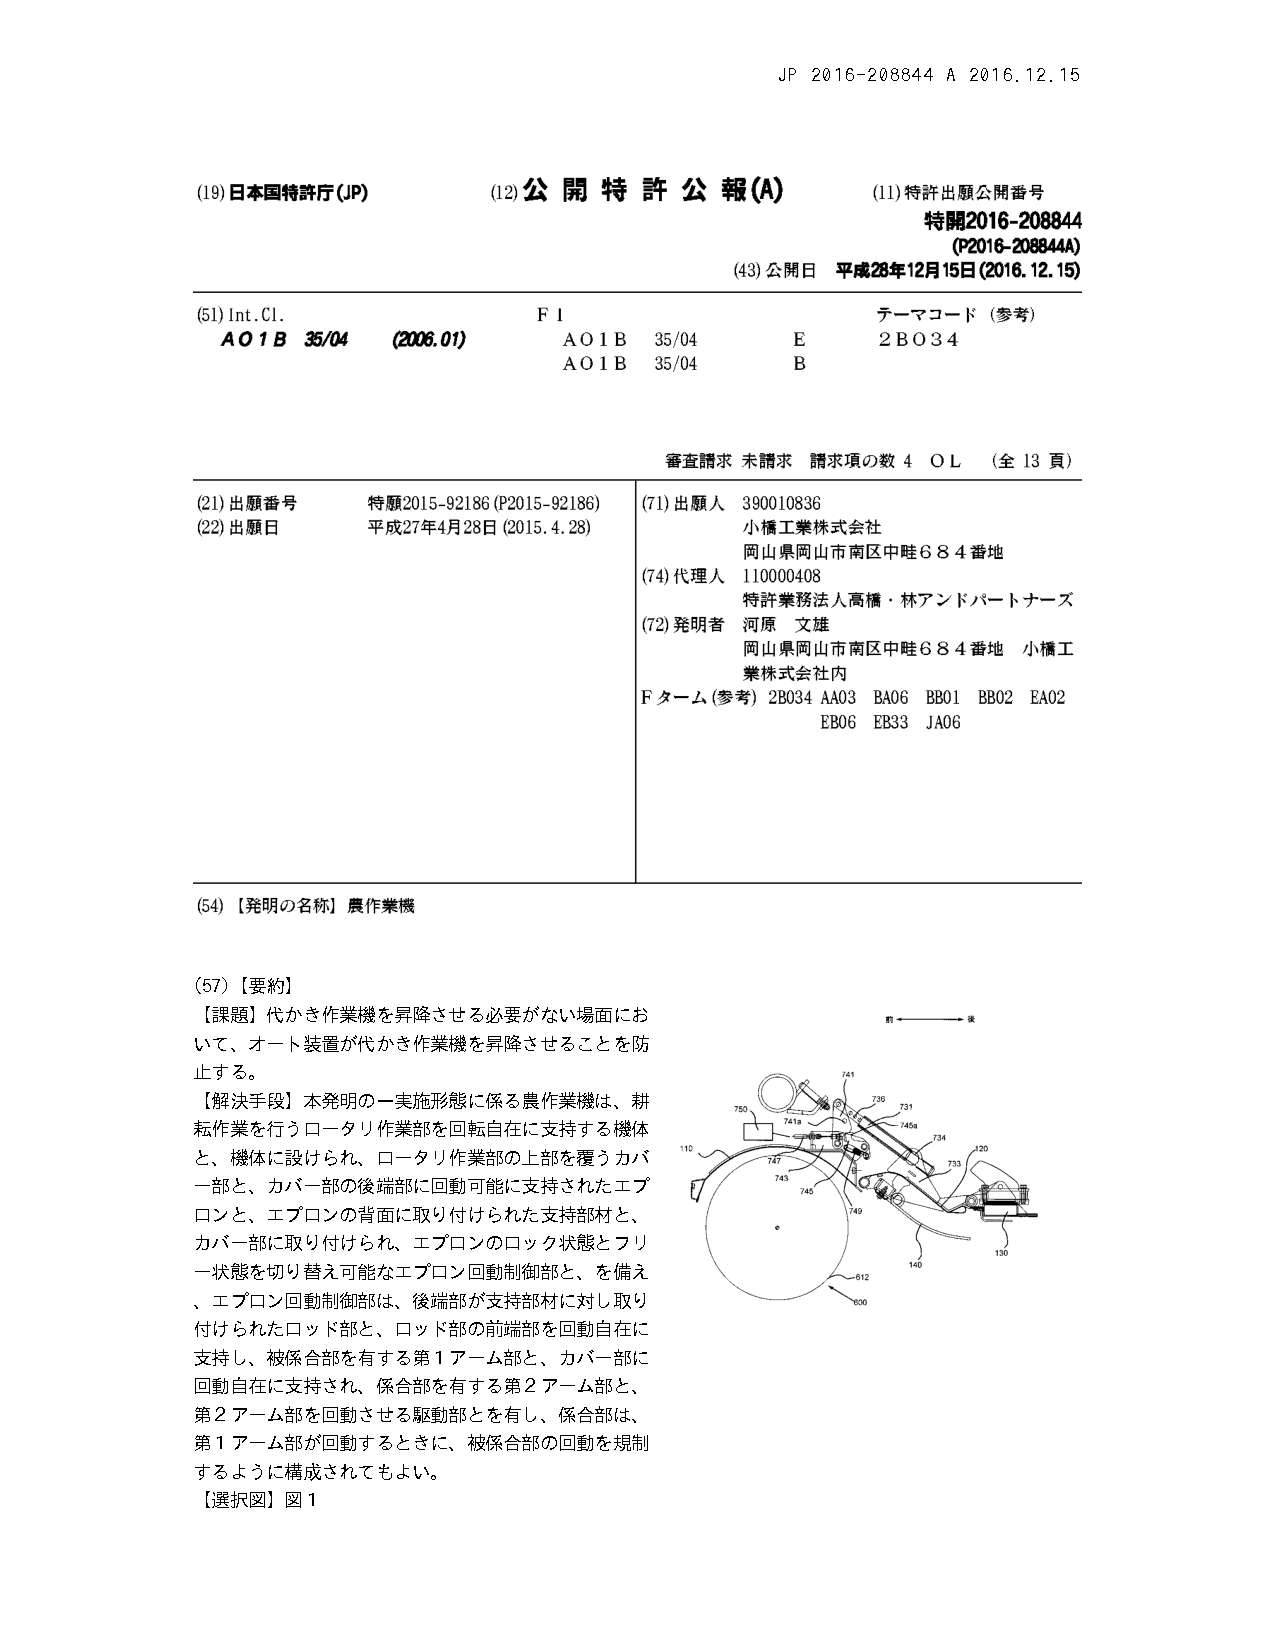
\includegraphics[width=0.9\textwidth,bb= 92 67 520 760]{ex1-1.pdf}
   \caption{特許文書例(a)}
   \label{fig:expa}
 \end{figure}
 \begin{figure}
  %\hspace*{-2cm}
  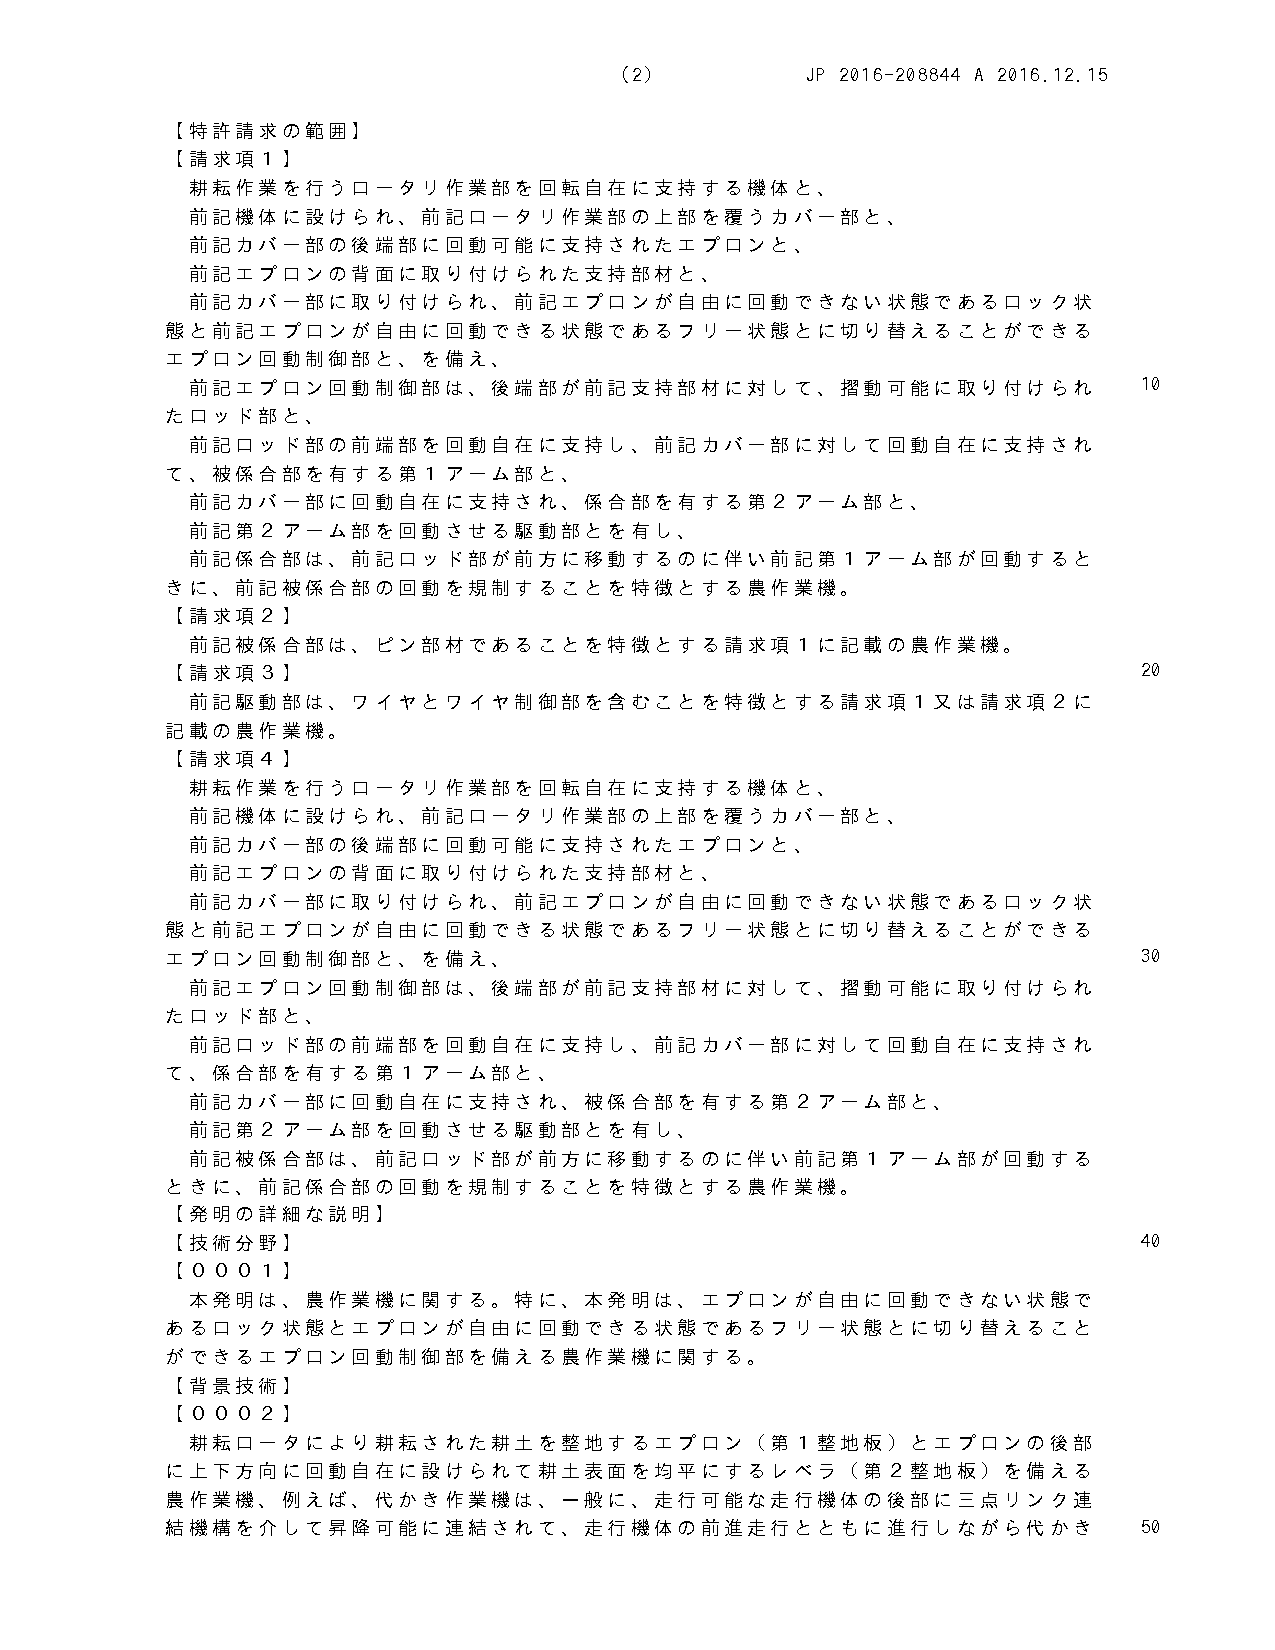
\includegraphics[width=0.9\textwidth,bb= 79 54 557 761]{ex1-2.pdf}
  \caption{特許文書例(b)}
  \label{fig:expb}
 \end{figure}

 図\ref{fig:expa},\ref{fig:expb}は特許文書の例である.
 発明の範囲を正確に記載するように請求項は普段に使わない学術用語を用いる. また,一般的な文書は単語をなるべく重複しないようにする一方,特許文書は単語を全体を通じて統一して使用し,指示代名詞はなるべく用いない.
 そのため,特許データベースでは一般的なウェブ文書データベースより多くの単語があり,単語の曖昧性が少ない.
 
 \section{特許分類}
 特許では人手によって分類され,特定の分類コードが付いている.
%特許分類を用いることより検索する特許文書が減り,似たようなキーワードを含むが分類が違う特許文書を排除することができる.
 今,最も使われている特許分類が世界知的所有権機関(WIPO)によって管理されている国際特許分類(IPC)である.
 IPCは世界標準であるため,同じ分類コードが付いているどの国の特許も同じ分類に属する.
 国際特許分類は階層構造であり,一番上の階層はAからHまでの8個のセクションである.
 セクション以下は表\ref{tab:IPC}に表したように四つの階層に分類されている.
 
 \begin{table}[!hbp]
 \center
 \begin{tabular}{cc}
    セクション:A & 健康および娯楽 \\
    サブセクション : 61 & 医学または獣医学:衛生学 \\
    クラス: C & 歯科:口腔または歯科衛生 \\
    メイングループ:5 & 歯の充填または被覆 \\
    サブグループ:08 & 歯冠:その製造;口中での歯冠固定 \\
 \end{tabular}
 \caption{国際特許分類例:A61C 5/08}
 \label{tab:IPC}
 \end{table}
 
 一般に,1つの特許が複数の分類に属する.
 本論文で用いる特許データベースでは一件あたり平均2.4個の分類コードが付いている.
 本論文では特許発明の主体を表す筆頭コードをその特許が属する分類とする.
 
 \section{特許検索}
 特許データベースにおける検索は技術水準調査,新規性調査,無効資料調査と侵害調査に分けられる.
 表\ref{tab:type}では4つの検索タイプを検索対象あるいは検索質問の発端となるものと検索の目的を示す.
 本論文では特許の新規性調査における検索質問の安全性について分析する.
 新規性調査はまだ出願していない発明について検索するため,
 質問意図が漏れたら,
 自社の研究開発動向など企業秘密が知られ,
 攻撃者に先に出願される恐れがある.
 
 \begin{table}[!hbp]
 \center
 \begin{tabular}{|c|c|c|}
 \noalign{\hrule height 1pt}
 検索タイプ & 検索対象(specification) & 検索目的 \\
 \hline
 \tabincell{c}{技術水準調査\\(State of the Art Search)} & アイデア & 自分の発明に関連する背景知識を得る \\
 \tabincell{c}{新規性調査\\(Novelty Search)} & 特許願書 & 特許登録の可能性を判断する \\
 \tabincell{c}{無効資料調査\\(invalidity Search)} & 特定な特許 & 発明の特許性の有無を判断する \\
 \tabincell{c}{侵害調査\\(Infringement Search)} &  \tabincell{c}{商品と\\商品に関連する技術} & 権利侵害とならないかを判断する \\
 \noalign{\hrule height 1pt}
 \end{tabular}
 \caption{特許検索タイプ}
 \label{tab:type}
 \end{table}

 本論文ではNTCIR-6\cite{NTCIR6}で用いた特許文書集合と無効資料検索タスクの質問を用いて評価実験をする.
 無効資料調査の目的は第三者の発明に特許性がないことを示す根拠となる文書を検索することであるが,
 特定発明の特許性の有無を判断することは新規性調査と一致するため,
 無効資料検索タスクの質問を新規性調査の質問とすることが妥当であると考えられる.
 


 \chapter{曖昧化検索} \label{s:OBS}
 曖昧化検索は質問者が検索したい真の質問と質問者側で生成したダミー質問を1つの質問グループにし,検索サーバに提出し,真の質問がどれかを曖昧化するものである.
 本論文では以下のモデル\cite{obs2012}を用いて既存の曖昧化検索メカニズムを分析する.
 質問者Aliceがとある検索サーバに質問を入力して手に入れたい情報を検索し,
 検索サーバがsemi-honestな攻撃者であることを仮定する.
 Semi-honestな攻撃者はプロトコルには従うが,必要以上の情報を得ようと試みる.
 
 質問が単語の集合であり,質問の定義域を単語集合の冪集合にする.
 
 \begin{defi}{ユニバーサル質問集合$Q$.}
  $W$を全ての単語の集合とする.
  ユニバーサル質問集合$Q$とは$W$の冪集合である,つまり
  \begin{equation}
  Q = P(W) = \{A|A \subset W\}
  \end{equation}
 \end{defi}
 Aliceのプロフィールを多項分布と仮定し,Aliceが持つ真のプロフィールを$X$とする.
 
 \begin{defi}{質問者のプロフィール$X$.}
  $T$を全てのトピックの集合とする.
  質問者のプロフィール$X$とは
  \begin{equation}
   X = \{x_i| i \in T\}
  \end{equation}
  $x_i$は質問者がトピック$i$に対して持つ興味の強さを表す.
 \end{defi}
 曖昧化検索メカニズムはAliceのコンピュータで実行する.
 曖昧化検索メカニズムが意味分析ツール$SA$を用いて真の質問$q_R$を分析しダミー質問$q_D$を生成する.
 生成したダミー質問$q_D$と真の質問$q_R$を1つの質問グループにし,検索サーバに提出する.
 意味分析ツール$SA$を用いるとき質問$q$とトピック$t$の関係を表す関数は以下のように定義する,
 
 \begin{defi}{質問-トピックスコア関数:$rscore_{SA}$.}
  $T$を全てのトピックの集合とする.
  質問$q$とトピック$t$の関係を表す関数とは
  \begin{equation}
   rscore_{SA}:Q \times T \to \mathbb{R}
  \end{equation}
 \end{defi}

 \begin{defi}{質問$q$のメイントピック:$\delta_{SA}(q)$.}
  $T$を全てのトピックの集合とする.
  質問$q$のメイントピック$\delta_{SA}(q)$とは
  \begin{equation}
   \delta_{SA}(q) = \argmax_{t \in T} rscore_{SA}(q,t)
  \end{equation}
 \end{defi}

 次に質問$q$のトピックベクトルを定義する.
 質問$q$のトピックベクトル$tvec_{SA}(q) = (rscore_{SA}(q,t_1 ), \dots , rscore_{SA}(q,t_{|T|})$とは
 $q$と全てのトピック$t_i$の質問-トピックスコア関数$rscore(q, t_i)$を要素として持つ$|T|$次元ベクトルである.
 質問のトピックベクトルを使って質問間の関係を評価することができる.

 検索サーバがAliceからもらった質問をすべて記録し,その全質問を分析して得るプロフィールを$Y$とする.

 \begin{defi}{質問比較関数:$C$.}
  質問比較関数$C:Q \times Q \rightarrow \mathbb{R}$を以下のように定義する
  \begin{equation}
  C_{SA}(q_1,q_2) = \frac{(tvec_{SA}(q_1) \cdot tvec_{SA}(q_1))}{||q_1|| ||q_2||}
  \end{equation}
 \end{defi}
 
 
 曖昧化検索は3つ違うレベルの目標がある.
 まずは質問そのものの曖昧化である.
 質問者が検索した真の質問$q_R$はどの質問であるかをわからないようにする.
 2つ目は質問意図の曖昧化である.
 質問者が検索したいものは何であるかをわからないようにする.
 最後は質問者のプロフィール$X$の曖昧化である.
 $Y$から質問者が興味を持つトピックは何であるかをわからないようにする.
 
 質問の曖昧化ができたとしても質問意図の曖昧化ができると限らない.
 {林檎}と{リンゴ}の2つ質問から真の質問を確定することができないが,質問者が林檎について検索したいことが確定できる.
 同じように{林檎}と{梨}の2つ質問から質問者が検索したいを確定することができないが,質問者が果物に興味を持つことが確定できる.
 本論文では質問意図の曖昧化をメインにする.

 次に検索質問のプライバシー保護の代表的な手法,
 否認可能検索(PDS)\cite{providing2009},
 質問者のプライバシーを保護する質問加工法(ETSQ)\cite{embellishing2010},
 質問意図を曖昧化するキーワード検索(HDGA)\cite{masking2014}を紹介する.
 
 \section{否認可能検索}\label{s:PDS}
 否認可能検索という概念を提出したのは\cite{PDS2008}である.
 つまり, サーバは特定な質問者が特定の時間に提出した一連の質問$L = {q_1, q_2, \dots , q_K}$のログを持つと仮定する. 
 ログにアクセスしたある人が真の検索質問が$q_i$だと証明したいとき, $L$の中の任意の質問$q_j$が真の質問となる確率が等しく$1/K$だと証明できる.
 以下に否認可能検索を定義する.
 \begin{defi}{$k$-否認可能検索:}
 	質問$q$を質問者が入力した質問とする.ダミー質問生成システム$DGS$が$k$個の質問を含んでいる質問集合$DGS(q_u)=\{q_1, \dots , q_k\}$を出力しサーバに提出する.
	$DGS(q_u)$が以下の性質を持つなら,$DGS(q_u)$をPD-質問集合といい,$D$を$k$-否認可能検索という
	\begin{enumerate}
	\item $\exists q_i \in DGS(q_u),q_i$と$q_u$が意味的に近い
	\item $\forall q_j \in DGS(q_u),DGS(q_j) = DGS(q_u)$
	\item $\forall q_j \in DGS(q_u),q_j$が違うトピックに含まれる
	\item $\forall q_j \in DGS(q_u),q_j$が同じような尤もらしさを持つ
	\end{enumerate}
  \end{defi}
 PDSでは事前に文書集合から高頻度な単語と単語ペアをシード質問として抽出し,
 潜在意味分析(LSA)\cite{LSA1990}を用いてシード質問をトピック空間にマップし,
 トピック空間に距離が近いシード質問をクラスタリングして標準質問とPD-質問集合を構築する.
 検索する場合は,質問者が検索したい質問の代わりに
 事前に用意した標準質問集合からトピック空間において質問者が検索したい真の質問と最も近い標準質問が属するPD-質問集合をサーバに提出する.
 次にサーバから検索結果を得て,質問者側で真の質問を用いて検索結果をフィルタリングする.
 以下でこの流れを具体的に述べる.
 %潜在意味分析の詳細は第\ref{s:sm}章で述べる.
 \subsection{シード単語と標準質問}
 システムが生成した質問は通常は使わない単語の組み合わせを使うことがある.
 攻撃者がこのような質問をダミー質問と判定し,真の質問を特定する可能性があるため,PDSは標準質問とPD-質問集合を事前に構築する.
 そのため,$Q$の中の全ての質問をカバーすることは不可能である.
 PDSの目標は妥当な再現率を得ることであるため,高頻度な単語だけを使うことは適当だと考えられる.
 
 \begin{algorithm}
 \caption{標準質問の構築}
 \begin{algorithmic}[1]
  \Require シード質問集合$S$
  \State $Q_C \Leftarrow \phi$
  \State Kdtreeを構築し$S$の全ての要素を追加する
  \ForAll {$s_i \in S$}
  \State Kdtree を用いて$s_i$と最も近いシード質問$c_1,c_2$を選ぶ
  \State $cquery = s_i \cup c_1 \cup c_2$
  \If {$cquery \notin Q_c$}
  \State $Q_C = Q_C \cup \{cquery\}$
  \EndIf
  \EndFor
  \Ensure 標準質問の集合$Q_C$
 \end{algorithmic}
 \label{a:cq}
 \end{algorithm}

 まず,単語・文書行列に頻出パターンマイニング\cite{apriori2010}を用いて
 $\Delta$回以上に表れた単語と連続する単語からなる単語ペアをシード質問として抽出し,トピック空間にマップする.
 シード質問は質問者の意図を適切に表さないことが多いため,
 PDSでは意味的に近いシード質問をグループにして標準質問にする.
 アルゴリズム\ref{a:cq}ではこの流れを具体的に説明する.
 このステップの計算量は$O(NlogN)$となる.
 ここで$N$はシード質問の数である.

 \subsection{PD-質問集合の構築}
 PD-質問集合を構築するには,トピックは異なるが尤もらしさが近い標準質問を同じ質問集合に集めれば良い.
 そのため,多様性と尤もらしさを計算する方法を提案する必要がある.
 多様性ではトピック空間の中の距離で評価する.
 人間が作った質問と比較するため,合理的な大きさを持つ質問ログ$Q_L = \{q: q \in Q\}$にアクセスできると仮定する.
 $Q_C$と同様に$Q_L$もトピック空間にマップし,標準質問の近傍の中の$Q_L$の要素数で標準質問の尤もらしさを計算する.
 近傍に多くの$Q_L$に含まれる質問がある標準質問を尤もらしさが高いとする.

 次に3つの部分の和となる標準質問間の関係を評価する関数を定義する.
 質問$q_1$と質問$q_2$のユークリッド距離$edist(q_1,q_2)$とは,
 \begin{equation}
 edist(q_1,q_2) = \sqrt{\sum_{i \in T}(tvec_{LSA}(q_1)[i] - tvec_{LSA}(q_2)[i])^2}
 \end{equation}
 である.
 ユークリッド距離が大きい質問が異なるトピックに含まれると考えられる.
 質問$q$の強度とは,
 \begin{equation}
 ||q|| = \sqrt{\sum_{i \in T}(tvec_{LSA}(q)[i])^2}
 \end{equation}
 である.
 質問$q$の近傍中の質問数$nhc(q)$とは,
 \begin{equation}
 nhc(q) = count(tvec_{LSA}(q),Q_L,HCUBE(tvec_{LSA}(q),\vec(\delta)))
 \end{equation}
 である.
 ここで,$Q_L$は質問ログ,$HCUBE(tvec_{LSA}(q),\vec(\delta))$は$tvec_{LSA}(q)[i] \pm \delta[i]$となる超立方体であり,
 $count$は超立方体中で$Q_L$に属するベクトルの数を返す.
 
 \begin{defi}{質問間の評価関数:$dis$.}
  \begin{equation}
  	dis(q_1,q_2) = (1 - \frac{edist(q_1,q_2)}{\alpha}) + \frac{|||q_1|| - ||q_2|| |}{\beta} + \frac{|nhc(q_1) -nhc(q_2)|}{\gamma}
  \end{equation}
  ここで,$\alpha$は$Q_C$に属する全ての質問ペア間の最大のユークリッド距離,
  $\beta$は質問ペア間の最大の強度差で,
  $\gamma$は質問ペア間の最大の近傍中の質問数の差である.
 \end{defi}
 
 したがって,近傍中の質問数と強度の差が小さく,
 トピック空間中の距離が大きい質問ペアの評価関数の値が低くなり,
 一つのPD-質問集合に入れるべきである.

 次では,質問集合間の評価関数を定義する.
 $A = {a_1, \dots , a_n}$と$B = {b_1 , \dots , b_m}$を2つ質問集合とする.
 $A$,$B$間の評価関数とは,
 \begin{equation}
    dis(A,B) = (1 - \alpha_1 / \alpha) + \beta_1 / \beta + \gamma_1 \gamma
 \end{equation}
 である.
 ここで,$\alpha_1 = \min_{i,j}(edist(a_i,b_j))$は2つの質問集合に属する質問ペア間のユークリッド距離の最小値であり,
 $\beta_1 = |\frac{\sum_i||a_i||}{n} - \frac{\sum_j||b_j||}{m}|$と
 $\gamma_1 = |\frac{\sum_inhc(a_i)}{n} - \frac{\sum_jnhc(b_j)}{m}|$は質問集合の強度と近傍中の質問数の平均の差である.
 
 \subsection{凝集型クラスタリング}
 PDSでは,まず質問ペアを要素とするレベル1集合$L_1$を生成する.
 $Q_C$に属する全の質問ペア間の評価関数の値の行列を計算し,
 評価関数の値が小さい順で質問ペアを$L_1$に加える.
 質問ペア$(q_i,q_j)$に対し,$q_i$か$q_j$ は評価関数の値がもっと小さいペアに属する可能性がある.
 その場合,$q_i$か$q_j$がすでに$L_1$にあることとなり,次に評価関数の値が小さいな質問ペアを選ぶ.
 選んだ質問ペアをマージし,次のレベルの集合($L_2,L_3, \dots$)を作る.
 マージステップはレベル変数$l$が$log_2k$になるまで続ける.
 したがって,最終レベルの集合中の質問クラスターの大きさが$k$となり,オーバーラップがないと保証する.

 \subsection{PD-質問集合の使用}
 真の質問$q_u$に近い標準質問を探すため,
 $q_u$をLSAを用いてトピックベクトル$tvec_{LSA}(q_u)$にし,
 質問比較関数$C(q_u,q_c)$が一番大きい標準質問$q_c$を選び,
 $q_c$が属するPD-質問集合をサーバに提出し,
 質問者側で真の質問を用いて検索結果をフィルターする.
 一定の再現率を得るため,普段の検索より多くの文書を手に入れる必要があるが,フィルターステップがこの影響をなくす.

 真の質問の全ての単語がPD-質問集合を構築するために使った単語リストに含まれていないなら,
 真の質問をLSAを用いてトピックベクトルにすることは不可能である.
 しかし,単語量が十分大きいなら,そのような状況が発生する可能性は低いと考えられる.
 また,(十分大きな)単語リストに含まれてない単語は質問者の意図を漏洩するリスクが高い.
 質問者がそのような質問を提出したとき,質問者に危険性を警告し,検索しないようにすることが考えられる.

 \section{質問者のプライバシーを保護する質問加工法} \label{s:ETSQ}
 今,テキスト検索サーバの大半が類似検索である.
 全ての質問単語を含んでいる文書しか検索できないキーワード検索と違い,
 類似検索は文書と質問の関連性を計算し文書にスコアをつける\cite{if2006}.
 毎回全ての文書との関連値を計算しないために,
 検索サーバが単語と文書の類似度を転置ファイルに保存し,
 質問の単語と文書の類似度の和を質問とその文書の関連値とする.
 このような計算が必要であるため,\cite{pss2006,opf2005,pke2004,soe2000}などキーワード検索しか対応できない研究は類似検索に応用できない.

 PDSをはじめに多くの曖昧化検索メカニズム\cite{masking2014,praw2005,goo2009}は質問の全体を分析し,適切な$K−1$個のダミー質問を選ぶ.
 質問の全体ではなく単語ごとにダミー単語を混ぜれば,
 真の質問である可能性がある質問数が増え,攻撃者が真の質問を見破る確率が下がる.
 質問者が1つのトピックに対して検索するとき,1つの単語を複数回使うと考えられる.
 毎回違うダミー単語を混ぜると同じ質問者の質問に出現する頻度が高い単語が真の質問単語となる可能性が頻度が低い単語より大きくなる.
 そうしたリスクを防ぐためETSQは単語バケットを事前に作り,真の質問単語と同じバケットにある他の単語をダミー単語とする.
 また,単語ごとにダミーを混ぜるため長い質問と類似検索に対応できる.

 \subsection{類似検索}
 コーパス$D$における検索サーバが質問を処理するとき基本的には転置ファイルを用いている.
 転置ファイルは質問単語の集合$W$と全ての単語の転置リストからなる.
 単語$w_i \in W$の転置リスト$L_i$が$\langle d_i,p_{ij}\rangle$の列である.
 $p_{ij} \in \mathbb{R}$は単語$w_i$と文章$d_i \in D$の関連値である.
 $w_i$が$d_i$に現れたなら$p_{ij}$の値は$0$より大きい,現れなかったなら$0$となる.
 空間圧縮のために$p_{ij}=0$な$d_i$は$L_i$に含まれていない.

 質問$q=\{w_i\}$と文書$d_i$と関連値は以下のように計算する
 \begin{equation}
 Score_{d_j,q} = \sum_{w_i \in q}p_{ij}
 \end{equation}
 したがって,転置リスト$L_i$に含まれている文書だけが$0$より大きいのスコアを持ち,$q$と関連があると見なす.
 転置ファイルを全体暗号化しても,サーバは転置リストの長さとアクセス頻度などの情報から真の関係値を推定できるため,
 そのような方法は無意味だと考えられる.
 
 \subsection{単語バケット}
 単語バケットを作るには2つ主要なリスクがある.
 真の質問単語が全て同じトピックについて述べると考えられる.
 そのような単語がランダムに選んだダミー単語と区別することが簡単である.
 また特許検索に多く使っている専門用語など特殊な単語と一般的よく使っている単語を混ぜると,専門用語が真の質問である可能性が大きいと考えられる.
 そんなリスクを減らすために,以下の特徴を持つ単語バケットを作りたい:
 \begin{enumerate}
 \renewcommand{\labelenumi}{(\roman{enumi})}
 \item 同じバケットにある単語の特殊さは近いが,意味的には大きい違いがある.
 \item 2つのバケットの全ての単語間の意味的距離の差が小さい.
 \end{enumerate}
 検索するとき,質問単語が属するバケット中の他の単語がダミー単語として質問に加える.
 したがって,特殊な単語のダミー単語がいつも同じような特殊さを持ち,ダミー単語間の関係と真の質問の単語間の関係が似ていると考えられる.

 紹介文献では単語を類義関係のセット(synset)でグループ化し,一つのsynsetが一つの概念に対応し,
 各synsetは上位下位関係,全体部分関係などの関係でリンクされているWordNet\cite{wordnet1995}を用いて単語バケットを作る.

 2つの単語が属するsynset間の最短パスを単語間の意味的距離とする.
 また上位下位関係でリンクされた2つsynsetの中下位語が上位語より特殊であると考えられる.
 WordNetの中で実体(entity)以外全部の名詞synsetの上位語が唯一に存在する.
 上下位関係を枝とすると,WordNet中の名詞synsetが実体を根とする木となる.
 単語が属する一番深さが浅いsynsetの深さを単語の特殊レベルとし,レベルが大きければ大きいほど単語が特殊である.

 \subsection{バケット作り}
 本節では単語バケットを作る方法を述べる.
 まず,アルゴリズム\ref{a:bkt}を用いてWordNetデータベース中の意味的に近い単語を隣にして全ての単語一列に並べる.
 リンクが多いsynsetが意味的に豊富であるため,単語を一列に繋がる種として使われ,synsetの関係数が大きい方から小さい方への順で処理する.
 複数の意味を持つ単語が属する各synsetが意味的に近いと考えられ,同じ単語を持つsynsetを隣に並べる.
 また反意関係,上位下位関係,全体部分関係を持つsynsetを隣に並べる.
 2つの操作により,列に近い単語の意味も近いと保証する.

 WordNetデータベースにアルゴリズム1を行った結果データベース中全ての$117,798$個の名詞を一列に並べた.

 \begin{algorithm}
 \caption{単語を一列に並べる}
 \begin{algorithmic}[1]
 \Function{ProcessSynset}{synset ss}
  \If {$ss$の単語が複数の既存の単語列に含まれている}
   \State そんな単語列を結合する
   \State 結合した単語列を$sq$にする
  \ElsIf {$ss$の単語が既存の単語列に含まれていない}
   \State 新たの単語列を作る
  \Else {\, $ss$の単語の一つが一つ既存の単語列に含まれている}
   \State その単語列を$sq$にする
  \EndIf
  \State 処理していない$ss$の単語を$sq$に加える
  \State $ss$の単語を処理したとマークする
  \State $ss$を処理したとマークする
  \State 単語列$sq$を返す 
 \EndFunction
 \Function{SequenceVocab}{WordNet wndb}
  \State 全てのsynsetを関係数が多い方から小さい方への順で並べる
  \State 全てのsynsetを処理していないとマークする
  \State 全ての単語を処理していないとマークする
  \State $SeqSet = \phi$
  \ForAll {処理していないsynset $ss$}
   \State $sq=ProcessSynset(ss)$;$sq$を$SeqSet$に加える
   \ForAll {$ss$と反意関係,上位下位関係,全体部分関係をもつsynset $ss'$}
    \State 処理していない$ss'$の単語を$sq$に加える
    \State $ss'$の単語を処理したとマークする
    \State $sq=ProcessSynset(ss')$;$sq$を$SeqSet$に加える 
   \EndFor
  \EndFor
 \EndFunction
 \end{algorithmic}
 \label{a:bkt}
 \end{algorithm}

 \begin{figure}[!hbp]
  \centering
  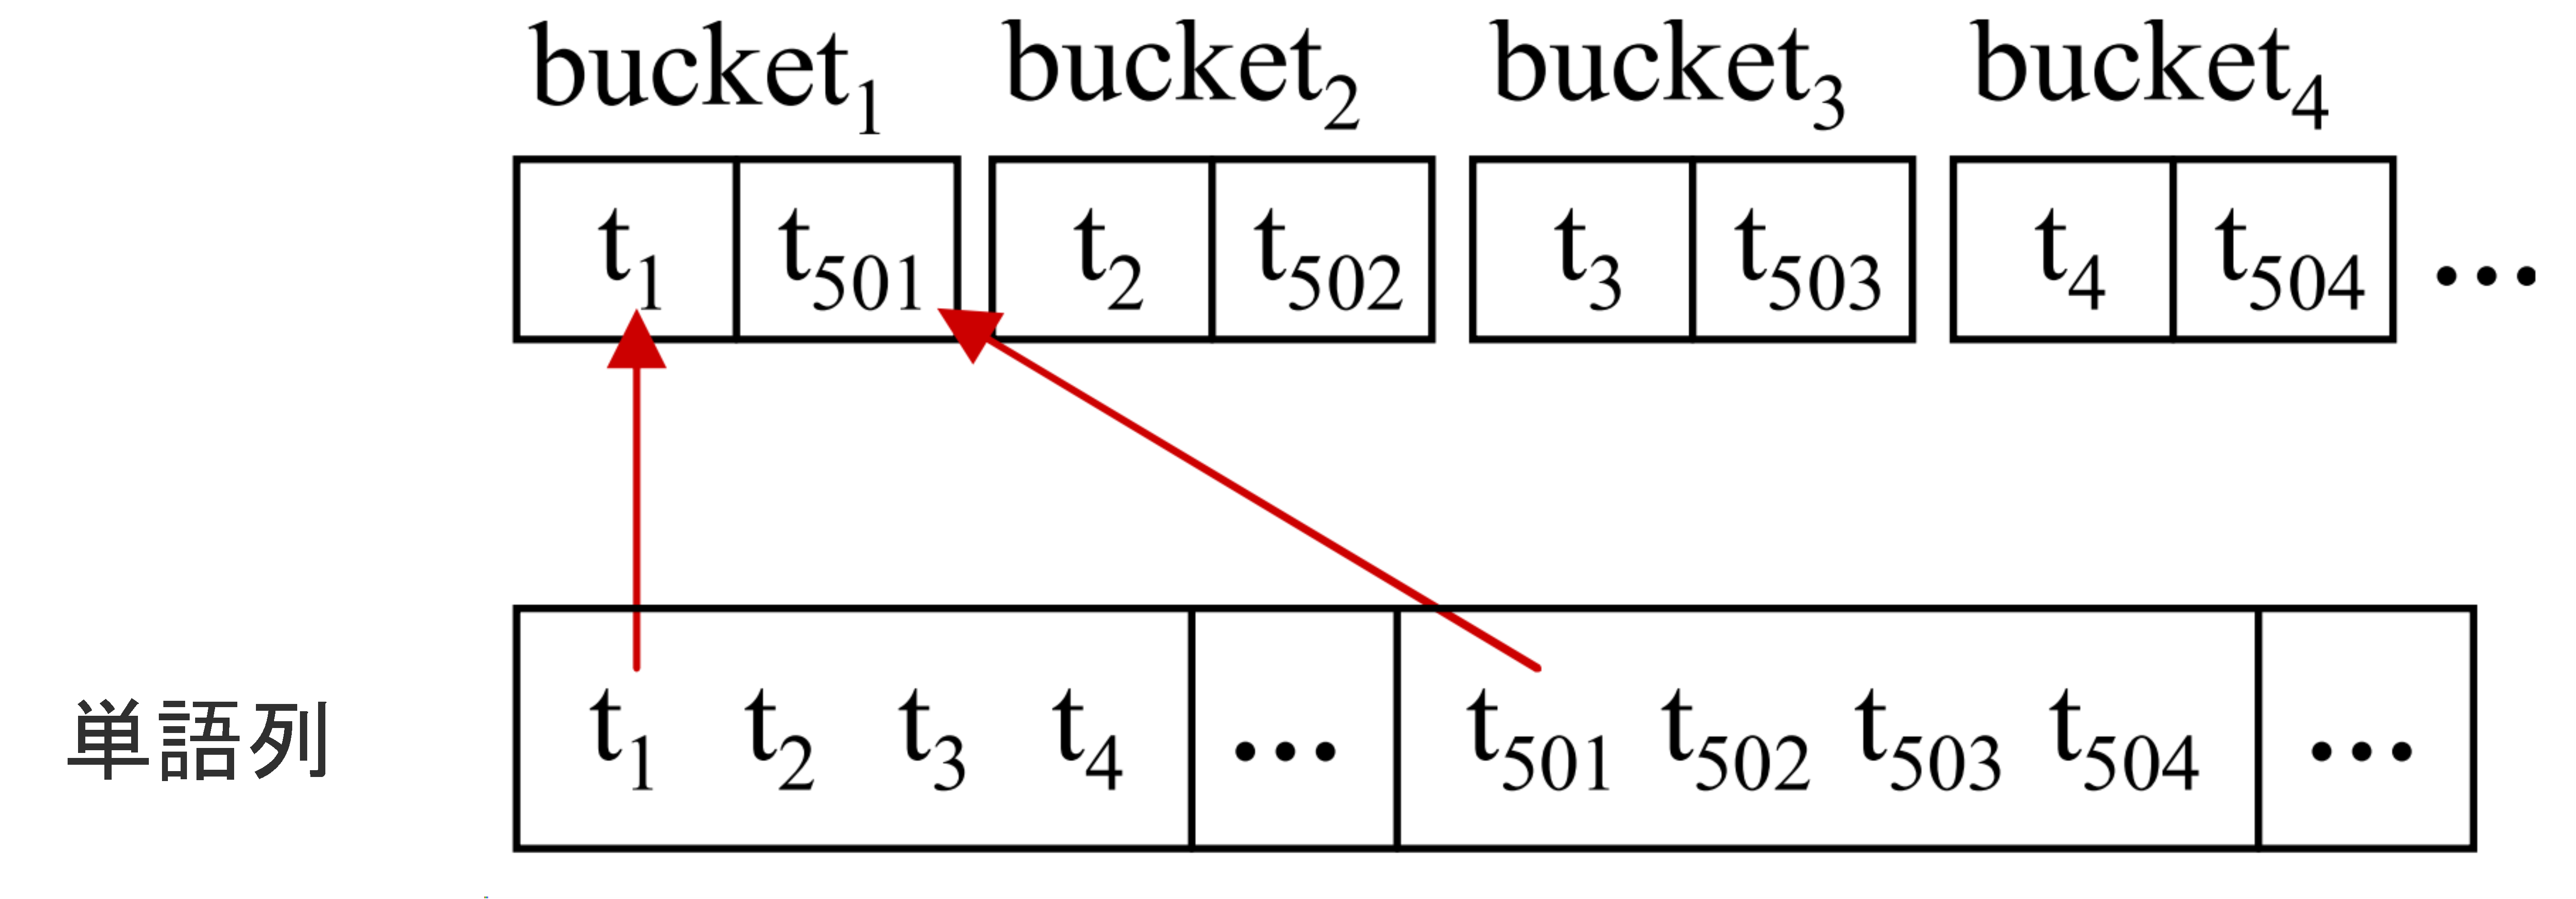
\includegraphics[width=0.8\textwidth,natwidth=5677,natheight=1982]{rk11.png}
  \caption{バケット作り-$N=1000,BktSz=2$}\label{fig:bkt}
 \end{figure}

 \begin{algorithm}
 \caption{単語列から単語バケットを作る}
 \begin{algorithmic}[1]
 \Function{GenerateBuckets}{sq,BktSz,Segsz}
  \State $N=$単語列$sq$の長さ
  \State $\#Seg=N/SegSz$
  \State $sq$を同じ長さのセグメントに分割する$S_1,S_2, \dots , S_{\#Seg}$
  \State セグメント中の単語を特殊レベルが大きい方から小さい方への順で再配列する
  \For {$i = 1 to N/(BktSz * SegSz)$}
   \State ActiveSeg = $\phi$
   \For {$j = 1 to BktSz$}
    \State $ActiveSeg = ActiveSeg \cup S_{(j-1)N/(BktSz * SegSz)}$
   \EndFor
   \For {$j = 1 to SegSz$}
    \State 新たなバケット$B=\phi$を作る
    \State ActiveSeg中の全てのセグメントの$j$番目の単語を$B$に入れる
    \State $B$を出力する
   \EndFor
  \EndFor
 \EndFunction
 \end{algorithmic}
 \label{a:bkt2}
 \end{algorithm}
 
 次ではアルゴリズム\ref{a:bkt}で出力した単語列を単語バケットにする.
 アルゴリズム2がその過程を表している.
 バケットの大きさBktSzを$1 \leq$BktSz$\leq N$に設定する.
 バケットの数が\#Bkts$=N/$BktSzである.
 同じバケット中の単語を可能な限りに違う意味にするために単語列の
 $1,\#$BktSz$+1,2*\#$BktSz$+1, \dots,($BktSz$-1)*\#$BktSz$+1$番目の単語をバケット$1$に,
 $2,\#$BktSz$+2,2*\#$BktSz$+2, \dots,($BktSz$-1)*\#$BktSz$+2$をバケット$2$に,
 $i,\#$BktSz$+i,2*\#$BktSz$+i, \dots,($BktSz$-1)*\#$BktSz$+i$をバケット$i$に入れる.
 図\ref{fig:bkt}が$N=1000,$BktSz$=2$のときのバケット作り過程を表している.
 その操作により,2つのバケット$i$と$j$の同じ位置の単語間の距離が同じ$\|i-j\|$であり,意味的な距離の差も小さいと考えられる.
 またバケット同じ位置の単語間の距離が違う位置の単語間の距離より近いため,真の質門の単語が同じ位置にあると仮定する.
 したがって,真の質問の単語が意味的に近いときあるいは一つのトピックに集中したとき,
 バケットの中のダミー単語も同じように一つのトピックに集中すると考えられる.
 しかし,バケット中の単語の特殊レベルがランダムであり,大きく違う可能性がある.

 バケット中の単語の特殊レベルを調整するために,隣接のバケット間の単語交換を行う.
 実際には単語を単語バケットに配置する前に単語列を同じ長さSegSz$\leq N/$BktSzのセグメントに分割し,
 セグメント内の単語を特殊レベルが大きい方から小さい方への順で再配列する.
 SegSzがBktSzの整数倍である必要がある.
 図\ref{fig:bkt2}が図\ref{fig:bkt}の上に単語列の再配列を加えた流れを表している.
 その結果,同じバケットにある単語のセグメント内の順番が同一であり,特殊レベルが近くなると考えられる.

 \begin{figure}
  \centering
  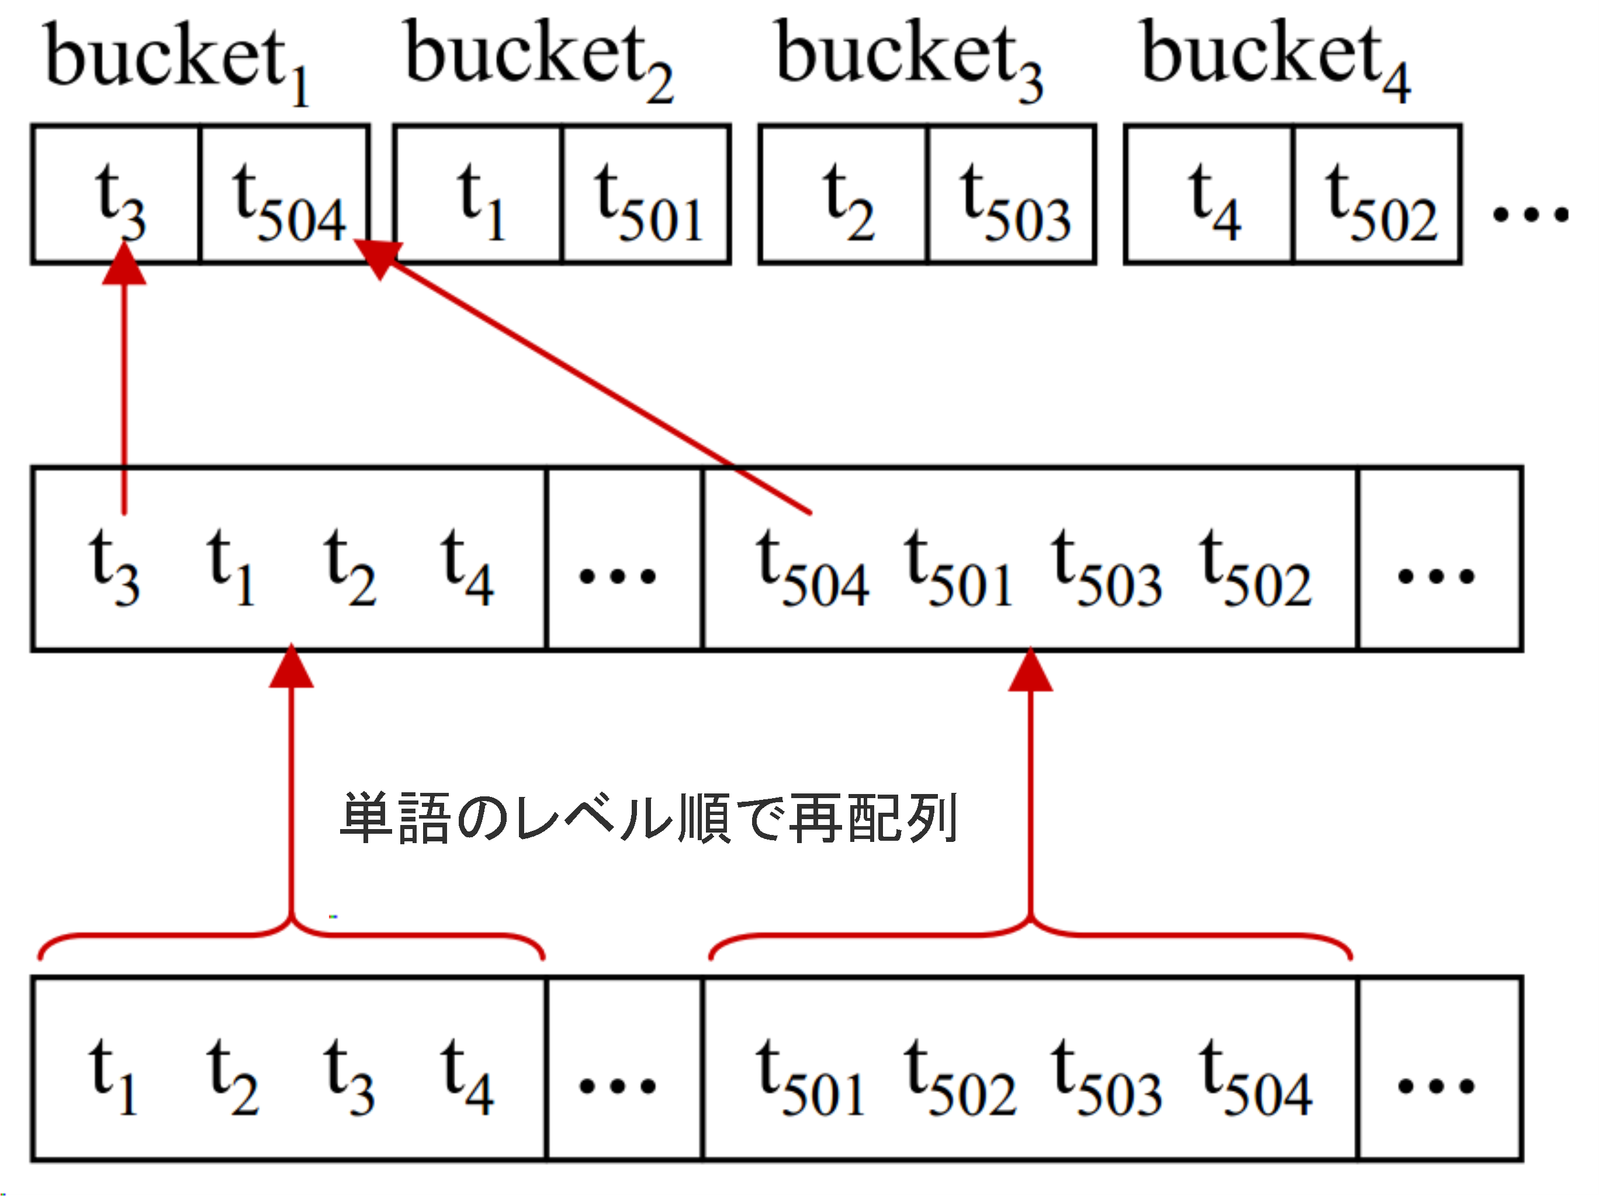
\includegraphics[width=0.5\textwidth,height=0.3\textwidth,natwidth=1600,natheight=1196]{rk13.png}
  \caption{バケット作り-$N=1000,BktSz=2,SegSz=4$}\label{fig:bkt2}
 \end{figure}

 バケット作りには2つのパラメータを設定する必要ある.
 SegSzが2つのリスクのトレードオフとなる.
 SegSzが増加することは単語交換を行う範囲が増大することに相当する.
 SegSzが大きければ大きいほどバケット中の単語の特殊レベルが近くなる.
 一方,単語間の意味的な距離も近くなる可能性がある.
 もう一つのパラメータBktSzがプライバシーと計算時間のトレードオフとなる.
 BktSzが大きくなると,真の質問を特定する可能性が下がるが,検索サーバが処理する質問単語が増加する.
 
 \subsection{プライベート検索スキーム}
 本節では真の質問単語だけの関連値を計算できる検索スキームを述べる.
 検索スキームは質問加工,質問検索と結果処理3つの部分からなる.

 \begin{algorithm}
 \caption{質問加工}
 \begin{algorithmic}[1]
 \Function{GenerateBuckets}{sq,BktSz,Segsz}
  \Require 真の質問単語$t_i$の集合
  \Ensure 加工した質問$q$
  \ForAll {真の質問単語$t_i$}
   \State Bkt$=t_i$が属する単語バケット
   \ForAll {$t_j \in $Bkt}
    \If {$t_i == t_j$} $\mu_j=1$
    \Else $\,\mu_j=0$
    \EndIf
    \State $E(u_j) = g^{\mu_j}\mu^r$
    \State $\langle t_j,E(\mu_j)\rangle$を$q$に入れる
   \EndFor
  \EndFor
 \EndFunction
 \end{algorithmic}
 \label{a:qe}
 \end{algorithm}

 アルゴリズム\ref{a:qe}が質問加工の流れを表す.
 真の質問単語が属するバケットの中の他の単語を全てダミー単語として質問に加える.
 ダミーを加えた質問の単語$t_j$に$E(\mu_j)$を付け,$t_j$が真の質問単語なら$\mu_j=1$,ダミー単語なら$\mu_j=0$.
 $E(\cdot)$は加算可能な準同型暗号\cite{dpe1994}の暗号化関数である.
 加算可能な準同型暗号が以下2つの特徴を持つ.
 二つの暗号文$E(m_1), E(m_2)$が与えられたときに,平文や秘密鍵なしで$E( m_1 + m_2 )$を計算できる.
 また,同じメッセージ$m$が複数の暗号文に対応でき,攻撃者が暗号文の頻度から$m$を推定することを防げる.

 \begin{algorithm}
 \caption{質問検索}
 \begin{algorithmic}[1]
 \Function{GenerateBuckets}{sq,BktSz,Segsz}
  \Require 加工した質問$q$
  \Ensure 文書とその文書暗号文した関連値の集合$R$
  \State $R=\phi$
  \ForAll {$\langle t_i,E(\mu_i)\rangle \in q$}
   \ForAll {$\langle d_j,p_{ij}\rangle \in L_i$}
    \If {$\exists \langle d_j,E(score_j)\rangle \in R$}
     \State $E(score_j)=E(score_j)*E(\mu_j)^{p_{ij}}$
    \Else
     \State $\langle t_j,E(\mu_j)^{p_{ij}}\rangle$を$R$に入れる
    \EndIf
   \EndFor
  \EndFor
 \EndFunction
 \end{algorithmic}
 \label{a:qs}
 \end{algorithm}

 アルゴリズム\ref{a:qs}がサーバ側の検索過程を表す.
 サーバが単語と文書の関連値を保存している転置ファイルを用いて文書の関連値を計算する.
 加算可能な準同型暗号の特徴より,$E(\mu_j)^{p_{ij}}=E(\mu_j*p_{ij})$.
 $t_j$がダミー単語であれば,$E(score_j)*E(\mu_j)^{p_{ij}}=E(score_j)*E(0*p_{ij})=E(score_j)$.
 復号した関連値には影響を与えない.
 したがって,$score_j$が真の質問単語と文書の関連値$p_{ij}$の和となる.

 最後に質問者がサーバがらもらった結果集合の関連値を質問者だけが持っている秘密鍵で復号し,
 その値を用いて文書を再配列するとプライバシー保護手法を使っていない検索サーバと同様な検索結果がもらえる.

 \section{質問意図を曖昧化するキーワード検索} \label{s:HDGA}

 HDGAは\cite{oti2012}提案した潜在ディリクレ配置法(LDA)\cite{lda2003}に基づく質問意図の曖昧化メカニズム(TIO)の改良手法である.
 LDAの詳細は第\ref{s:sm}章で述べる.
 HDGAが以下の特徴を持つ,
 まず,サーバに提出した質問グループに属する各質問が違うトピックに属し,ダミー質問の生成過程が相互独立である.

 次に,HDGAはTIOのように真の質問をカバーできるトピックからダミー質問を作るのではなく
 同じ質問グループに属する質問が同じ地位を持つようにする.

 そして,HDGAがハッシュ関数Highest Random Weigh(HRW)\cite{hrw1998}を用いてダミートピックを選び,トピックの出現頻度を均一にする.

 \begin{algorithm}
 \caption{HDGA(On Masking Topical Intent in Keyword Search)}
 \begin{algorithmic}[1]
  \Require 質問:$q_1$
  \State $Q = \{q_1\}\delta_{q_1} = \argmax_{t \in T} Pr[t|q_1]$
  \ForAll {$t \in T \setminus \{\delta_{q_1}\}$}
  \State $e_t = h(\delta_{q_1}||t||s)$
  \EndFor
  \State $T_D = \{t^1_{q1},t^2_{q1}, \dots , t^2_{q1} | \forall t_1 \ \in T_D , \forall t_2 \ \in T \setminus T_D, e_{t_1} > e_{t_2} \}$
  \ForAll {$t \in T_D $}
  \While { $ \argmax_{t \in T} Pr[t|q'] \neq t$}
  \State $Pr[w|t]$に基づいて$|q_1|$個の単語をランダムに選び,ダミー質問$q'$を作る
  \EndWhile
  \State $Q = Q \cup \{q'\}$
  \EndFor 
  \State $Q$をシャッフルする
  \Ensure $Q$
 \end{algorithmic}
 \label{a:HDGA}
 \end{algorithm}

 アルゴリズム\ref{a:HDGA}がHDGAの質問生成メカニズムを表す.
 ここで$Pt[w|t]$がLDA分析の結果であり,$h$がHRWハッシュ関数である.

 \chapter{意味分析} \label{s:sm}
 第\ref{s:OBS}章で述べたように質問意図を隠せるダミー質問を作るために
 質問が持つ意味を計算機に理解させなければならない.
 まず,文書や質問などをベクトルで表す必要がある.
 自然言語研究で多く使用されるベクトル表現方法がbag-of-wordsである.
 bag-of-wordsとは単語を袋に入れるように,単語の出現順番などの情報を捨て,
 単語の出現頻度だけをベクトル要素とする表現方法である.
 次に質問が持つ意味を数字にすると,
 質問をトピックベクトルで表現できる.
 したがって,質問が持つ意味を数字にすることは
 質問を記述するために必要な次元数を減らすことであると考えられる.
 情報検索分野ではコーパス中の文書を記述するために必要な次元数を減らす研究を進めている.

 $tf\text{-}idf$はが単語とコーパス中の文書の関連値を実数値で表せるため,
 文書数$|D| \times$単語数$|W|$の行列$M$でコーパスを記述できる.
 潜在意味分析(LSA)は行列$M$を特異値分解(SVD)し低ランク近似し,より高い圧縮を得る.
 しかし,LSAモデルのパラメータ数がコーパス中の文書数の共に増加するためオーバーフィットの恐れがあり,
 コーパスに含まれていない文書を記述する方法が明らかにさせていない.
 そのような問題を解決するために確率モデルである潜在ディリクレ配置法(LDA)が提案された.

 本論文ではこの3つの意味分析手法を全て用い,
 評価実験をする.
 以下では上記意味分析手法を紹介する.

 \section{tf-idf}
 コーパス中に含まれている文書の集合を$D$とし,
 単語$w_i$の文書$d_j$における出現回数を$n_{i,j}$とする.
 単語$w_i$の文書$d_j$における出現頻度を
 \begin{equation}
 tf_{i,j} = \frac{n_{i,j}}{\sum_k n_{k,j}}
 \end{equation}
 単語$i$の逆文書頻度を
 \begin{equation}
 idf_i = log \frac{|D|}{|d|w_i \in d, d \in D|}
 \end{equation}
 と定義し,
 \begin{equation}
 tfidf_{i,j} = tf_{i,j} \cdot idf_i
 \end{equation}
 によって単語$t_i$の文書$d_j$における$tf\text{-}idf$値を計算する.
 
 本論文では国際特許分類を用い特許データベースに属する文書を$632$個の分類にし,
 各分類をトピックとし,
 \begin{equation}
 tfidf_{i,k} = \sum_{d_j \in t_k}tf_{i,j} \cdot idf_i
 \end{equation}
 によって単語$t_i$のトピック$t_k$における$tf\text{-}idf$値を計算する.
 人手により分類されている国際特許分類をトピックにしたため,
 各トピックの意味が明らかである.

 \section{潜在意味分析} \label{s:LSA}
 特異値分解(SVD)を用いて単語をトピック空間にマップすることが潜在意味分析の基礎である.
 LSAではトピック空間中の単語と文書の関係を用いて多義性と同義性の問題を解決する.
 つまり, 綴りが違うが同じような意味を持つ単語はトピック空間での距離が近いようにできる.

 単語$\times$文書行列$M$の$(i,j)$番目の要素は単語$w_i$のが文書$d_j$における$tf\text{-}idf$値である.
 $M$を特異値分解$M = USV^T$し,$U$,$S$,$V$ の各列ベクトルを特異値が大きい順に$K$個用いて$G$の低ランク近似$G_K=U_KS_KV_{K}^T$を得る.
 このように低ランク分解によって,単語とトピックの関係を分析できる.
 $M_K$の$(i,j)$番目の要素は$i$番目の単語と$j$番目のトピックの関係を表す.
 その値が大きければ大きいほど単語とトピックの関係が強い.
 単語$w_i$と対応する行列$M_K$の行$\ell_i$を単語$w_i$のトピックベクトルとし,
 \begin{equation}
 rscore_{LSA}(q,t_j) = \sum_{w_i \in q}\ell_i[j]
 \end{equation}
 によって質問$q$とトピック$t_j$の関連値を計算する.
 
 本論文では単語$\times$文書行列$M$の代わりに単語$\times$国際特許分類行列$M'$を用いる.
 単語$\times$国際特許分類行列$M'$の$(i,j)$番目の要素は単語$w_i$の国際特許分類$t_k$における$tf\text{-}idf$値である.
 国際特許分類は特許データベースの大きさと関係なく一定であるため,
 文書数の増加によるオーバーフィットを防ぐ.

 \section{潜在ディリクレ配置法}\label{s:LDA}
 潜在ディリクレ配置法(LDA)は文書の確率生成モデルである.
 LDAでは文書が複数の潜在的トピックからランダムに生成されると仮定し,
 トピックをそのトピックごとに単語の出現頻度で表す.

 
 LDAではコーパス$D$に含まれている長さが$n_d$である文書$d$の生成過程を以下のように仮定する:
 \begin{itemize}
 \item {\em コーパス$D$における各潜在的トピック$t$を生成する}$\phi_{t} \thicksim Dir(\beta)$
 \item {\em トピック分布ベクトル$\theta_d$を生成する}$\theta_d \thicksim Dir(\alpha)$
 \item 各単語$w \in d$に対して:
  \begin{itemize}
   \item {\em $w$が属するトピック$t$を決める}$t \thicksim Mulinomail(\theta_d)$
   \item {\em $w$を決める}$w \thicksim Multinomial(\phi_{t})$
  \end{itemize}
 \end{itemize}
 
 ここで$\alpha,\beta$は$|T|$次元ベクトルで,Dirichlet分布のパラメータであり,
 $\theta_d,\phi_{t}$は確率ベクトルである.

 このグラフィカルモデルを図\ref{fig:LDA}に示す.
 \begin{figure}
 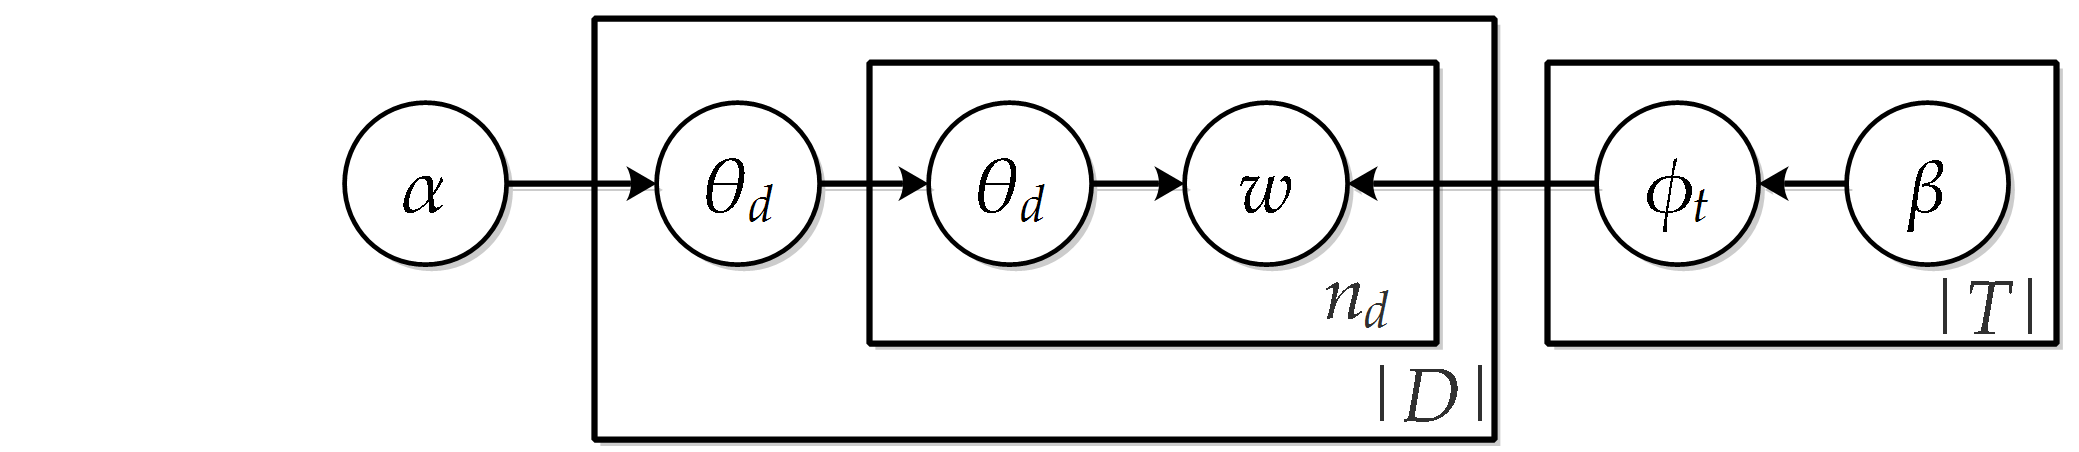
\includegraphics[width=0.9\textwidth,natwidth=557,natheight=141]{LDA.png}
 \caption{LDAのグラフィカルモデル}
 \label{fig:LDA}
 \end{figure}
 
 全ての文書が同じ確率を持つと仮定すると,
 \begin{equation}
 Pr[t] = \sum_{d \in D}\theta_{d,t}Pr[d] = \frac{\sum_{d \in D} \theta_{d,t}}{|D|}
 \end{equation}
 によってコーパス$D$の中の各トピックの確率を計算し,
 \begin{equation}
 rscore_{LDA}(q,t) = Pr[t|q] = \frac{Pr[q|t]Pr[t]}{Pr[q]} = \frac{\prod_{w \in q}Pr[w|t]Pr[t]}{\sum_{t \in T}\prod_{w \in q}Pr[w|t]Pr[t]}
 \end{equation}
 によって質問$q$と各トピックの関係性を計算できる.


 \chapter{攻撃手法}
 本論文では攻撃者が質問者が質問意図を隠していること
 と
 質問者が用いている質問曖昧化手法のメカニズムを知っているを前提とし,
 攻撃手法を考える.

 曖昧化検索は3つの違うレベルの目標があると同じように
 曖昧化検索に対する攻撃手法も3つの違うレベルの目標がある.
 1つ目の攻撃手法ではダミー質問が混ぜられた質問グループから真の質問$q_R$を見つける.
 2つ目の攻撃手法ではダミー質問が混ぜられた質問グループから質問者が検索したいものを見つける.
 3つ目の攻撃手法ではダミー質問が混ぜられた質問ログから質問者が興味を持つトピックを見つける.

 1つ目の目標に対して本論文では質問$q$と質問$q$のメイントピック$\delta_{SA}$間の関連値を攻撃するメイントピック攻撃を提案する.
 質問者が検索したいものを定義するのは難しいため,本論文ではダミー質問の検索結果と真の質問の検索結果が一致する割合を用いて評価する.
 そして,3つ目の目標を達成できる既存の攻撃手法類似度攻撃\cite{simattack2016}を紹介し,改良手法を提案する.

 \section{メイントピック攻撃}\label{s:MTA}
 HDGAなど真の質問とダミー質問を1つの質問グループにして提出する曖昧化手法対して,
 ダミー質問が真の質問と同様に全ての単語が1つのトピックに集中することが失敗したら,
 真の質問と真の質問のメイントピックの関連値が
 ダミー質問とダミー質問のメイントピックの関連値より強いと考えられる.
 メイントピック攻撃(MTA)は1つの質問グループの中で自分のメイントピックとの関連値が一番高い質問を
 真の質問とする.

 また,ETSQは真の質問単語ごとにダミー単語を混ぜ,1つの加工した質問にして提出する.
 関係が強い単語が他のトピックと関係が強い単語の数より多いと
 加工した質問のトピックと真の質問のトピックが一致することが考えられる.
 また,一つのバケットの中の単語が意味的に遠いため,
 ダミー単語が真の質問単語のメイントピックとの関連値が低いと考えられる.
 メイントピック攻撃では各単語バケット中質問のメイントピックと一番関連値が高い単語を真の質問の単語と推定する.

% \begin{algorithm}
% \caption{メイントピック攻撃}
% \begin{algorithmic}[1]
%  \Require 質問:$q=\{t_i\},$単語のトピックベクトル集合$L=\{\ell_i\}$
%  \State $R=\phi, \, \ell=0$
%  \State $\ell=\sum_{t_i \in Q}\ell_{t_i}$
%  \State $maintopic = \argmax_j \ell[j]$
%  \ForAll {$bk_k \in q $}
%  \State $R=R \cup \{\max_{t_i}l_{t_i}[maintopic]\}$
%  \EndFor \\
%  \Return $R$
% \end{algorithmic}
% \label{a:mt}
% \end{algorithm}

 \section{事前情報がある場合の類似度攻撃}\label{s:SimAtt}
 事前情報がある場合の類似度攻撃(SimAtt)\cite{simattack2016}は質問者が提出した質問と攻撃者が事前に得た質問者の質問ログ間の類似度を計算し,
 この類似度を用い質問者の新の質問を見破る.
 SimAttでは単語ベクトルで質問を表し,
 質問ログを質問の集合とする.
 アルゴリズム\ref{a:simatt}が質問$q$と質問者のログ$P_u$間の類似度$sim_{q,P_u}$の計算方法を示す.

 \begin{algorithm}
 \caption{類似度計算}
 \begin{algorithmic}[1]
  \Require 質問$q$,質問者のプロフィール$P_u$,スムージングパラメータ:$\alpha$
  \For {$q_i \in P_u$}
  \State $coef[i] \leftarrow 2 \cdot |q \cap q_i| \cdot \frac{1}{|q|+|q_i|}$
  \EndFor
  \State $coef \gets sort(coef)$
  \State $sim \gets coef[0]$
  \For {$i \in [1,|P_u|]$}
  \State $sim \gets \alpha \cdot coef[i] + (1 - \alpha) \cdot sim$
  \EndFor
  \Ensure $sim_{q,P_u}$
 \end{algorithmic}
 \label{a:simatt}
 \end{algorithm}

 ここで$coef[i]$は質問$q$と$P_u$に属する質問$q_i$間のDice係数\cite{dice1945}で,
 $\alpha$が重み係数である.
  
 \begin{algorithm}
 \caption{SimAtt}
 \begin{algorithmic}[1]
   \Require 質問グループ$G$,質問者のプロフィール$Pu$,スムージングパラメータ:$\alpha$
   \State $q^* = \argmax_{q \in Q}sim_{q,Pu}$
   \Ensure $q^*$
 \end{algorithmic}
 \end{algorithm}

 SimAttは質問グループの中質問者の質問ログと一番類似度が高い質問が真の質問であると判定する.
 攻撃方法は単純であるが,第\ref{s:ex}章の実験結果は特許データベースにおける攻撃の強さを示す.

 \section{事前情報がない場合の類似度攻撃} \label{s:SimAtt2}
 攻撃者が事前的に質問者の真の質問ログを持たないとSimAttを用いることができない.
 本節ではダミー質問を混ぜた質問ログのみから真の質問を見つける
 事前情報がない場合の類似度攻撃SimAtt2を提案する.
 質問者が同じトピックに対して複数の質問を提出することが考えられる.
 PDSなど真の質問と距離が大きい質問をダミー質問にする質問曖昧化手法では
 真の質問は同じトピック$t$に属するとしてもダミー質問は同じように別のトピック$t'$に属すると限らない.
 トピックの出現頻度から真の質問を見つけることができ,
 真の質問間の類似度がダミー質問間の類似度より高いと考えられる.
 HDGAはトピックの出現頻度を均一にできる.
 しかし,HDGAは$Pr[w|t]$に基づいて単語をランダムに選び,ダミー質問を生成するため,
 同じトピックに属するダミー質問間の距離が真の質問間の距離ほど近いと限らない.
 また,真の質問$q_1,q_2$が意味的に近いトピック$t_1,t_2$に属するとき,
 ダミー質問$q_1',q_2'$が属するトピック$t_1',t_2'$も意味的に近いと保証できない.
 したがって,意味的に近い一連の質問が真の質問である可能性が高いと考えられる.
 本論文では同じ質問者が提出した全ての質問グループから1つ質問を選び出した質問集合を質問列という.
 アルゴリズム\ref{a:simatt2}が意味的に近い質問列を取り出す攻撃手法を示す.

 \begin{algorithm}
 \caption{SimAtt2}
 \begin{algorithmic}[1]
  \Require 質問グループ列$\hat{G}=\{ G_1,G_2, \dots , G_m\}$,スムージングパラメータ:$\alpha$
  \For {$j \in |G_1|$}
   \State $\hat{Pu}[j] = G_1[j]$
   \State $\hat{Put}[j] = \Phi$
   \State $d[j] = 0$
  \EndFor
  \For {$i \in [2,m]$}
   \For {$j \in |G_i|$}
   \State $\hat{Put}[j] = \argmax_{Pu \in \hat{Put}}sim_{G_i[j],\hat{Put}[j]}$
   \EndFor
   \State $q^*_i = \argmin_{G_i[j] \in G_i}sim_{G_i[j],\hat{Put}[j]}$
   \For {$j \in |Q_i|$}
    \State $\hat{Pu}[j] = \hat{Put}[j] \cap G_i[j]$
   \EndFor
  \EndFor
  \Ensure $q^*$
 \end{algorithmic}
 \label{a:simatt2}
 \end{algorithm}
 
 SimAtt2は1つ質問グループに属する質問と同じ数の質問列$Pu$を可能な真の質問列として保存する.
 1つの質問グループに対してダミー質問を真の質問であると判定したとしても,
 その質問グループの中は必ず真の質問が存在するため,
 真の質問と真の質問と一番意味的に近い質問列が保存し,
 後続の質問グループに対する攻撃に利用される.
 したがって,
 SimAtt2について過去の攻撃ミスは後続の攻撃に影響しないと考えられる.


 \chapter{単語ベクトルを用いた質問曖昧化}

 \section{単語ベクトル}
 質問のメイントピック以外に質問に含まれている単語に情報も用いるため,
 本論文では単語ベクトルという概念を用いる.
 
 \begin{defi}{単語ベクトル.}
 $W$を全ての単語の集合とする.
 トピック$t$の単語ベクトル$wvec_{SA}(t)$とは
 $W$に属する全ての単語$w$を$w$と$t$の関連値を大きい方から小さい方まで並ぶ$|W|$次元のベクトルである.
 \begin{equation}
  wvec_{SA}(t)  = (w_1,w_2, \dots , w_{|W|})
 \end{equation}
 ここで次の(i), (ii)が成り立つ
 \begin{enumerate}
 \renewcommand{\labelenumi}{(\roman{enumi})}
 \item $\forall w \in wvec_{SA}(t), w \in W$ 
 \item $\forall 1 \leq i < j \leq |W|,w_i \neq w_j,rscore(w_i,t) \geq rscore(w_j,t)$
 \end{enumerate}
 \end{defi}

 質問のメイントピックを計算し,
 質問に含まれている単語をその単語が質問のメイントピックの単語ベクトル内での順番にすれば,
 質問を数字ベクトルで表わすことができる.
 同様にトピックが決めれば,
 そのトピックの単語ベクトルを用いて数字ベクトルを質問に翻訳することができる.
 すなわち,$index(w,vec)$をベクトル$vec$に元$w$の順番を返す関数とし,
 質問数字化関数$WtN$を
 \begin{equation}
  WtN_{SA}(q,t)  = \{index(w,wvec_{SA}(t))| w \in q\}
 \end{equation}
 によって定義する.
 また$atindex(n,vec)$をベクトル$vec$に順番が$n$となる元を返す関数とし,
 数字ベクトル質問化関数$NtW$を
 \begin{equation}
  NtW_{SA}(v,t)  = \{atindex(n,wvec_{SA}(t))| n \in v\}
 \end{equation}
 によって定義する.
 図\ref{fig:tv1},\ref{fig:tv1}はLDAを意味分析ツールとして用いるときの例を表している.

 \begin{figure}
 \begin{minipage}[t]{0.5\linewidth}
 \centering
 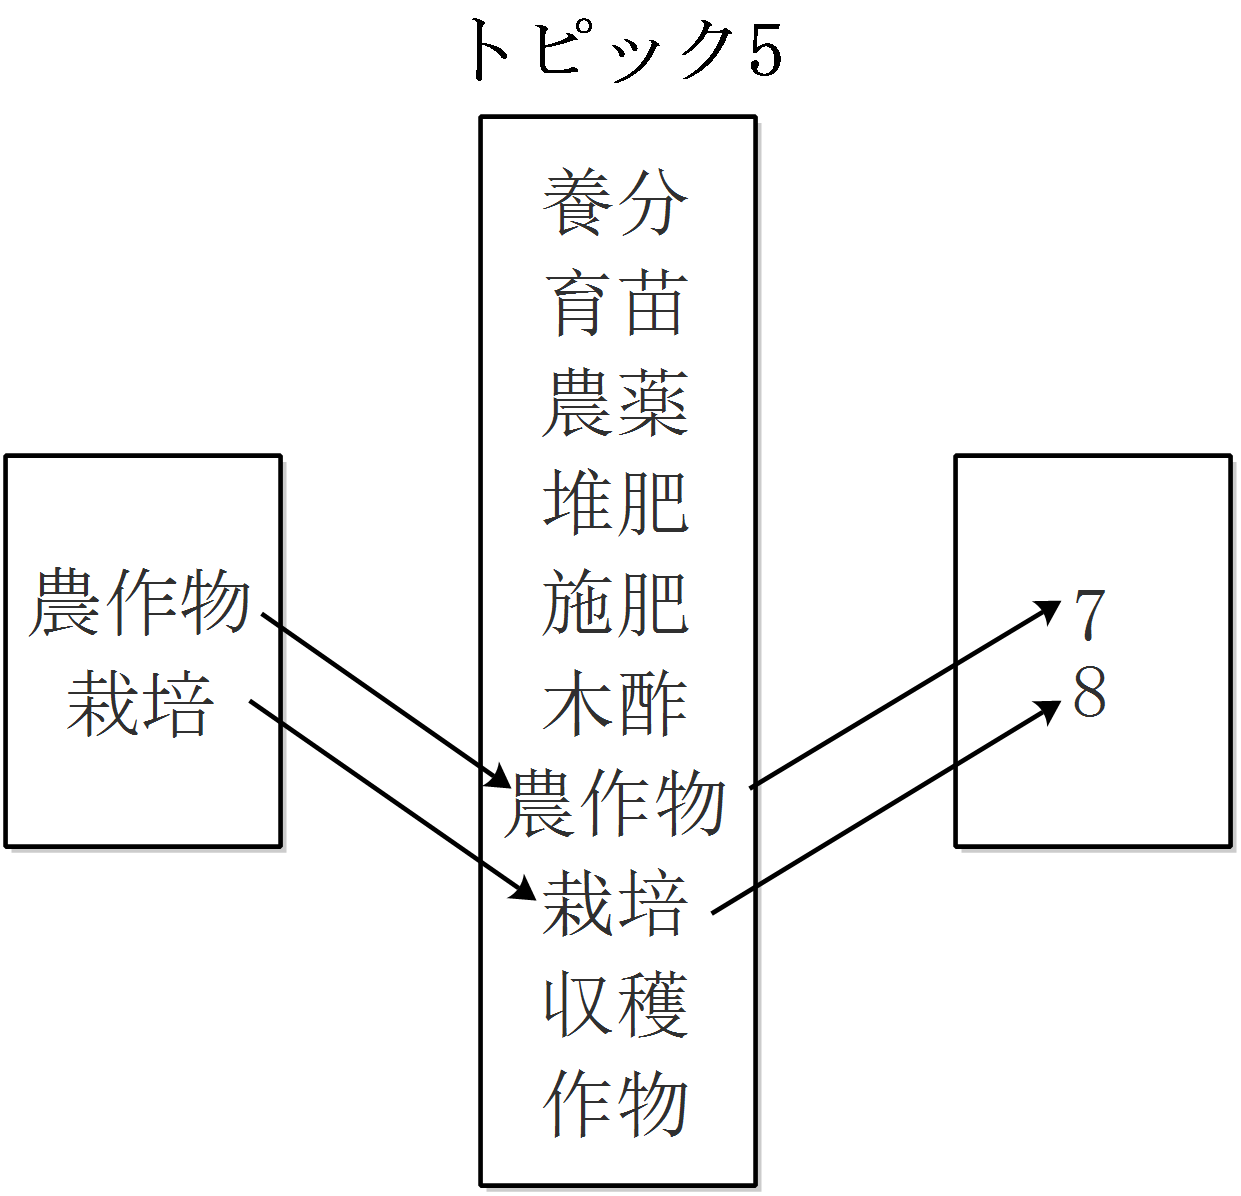
\includegraphics[width=0.9\textwidth,natwidth=310,natheight=299]{tv1.png}
 \caption{質問数字化関数$WtN$の例}
 \label{fig:tv1}
 \end{minipage}%
 \begin{minipage}[t]{0.5\linewidth}
 \centering
 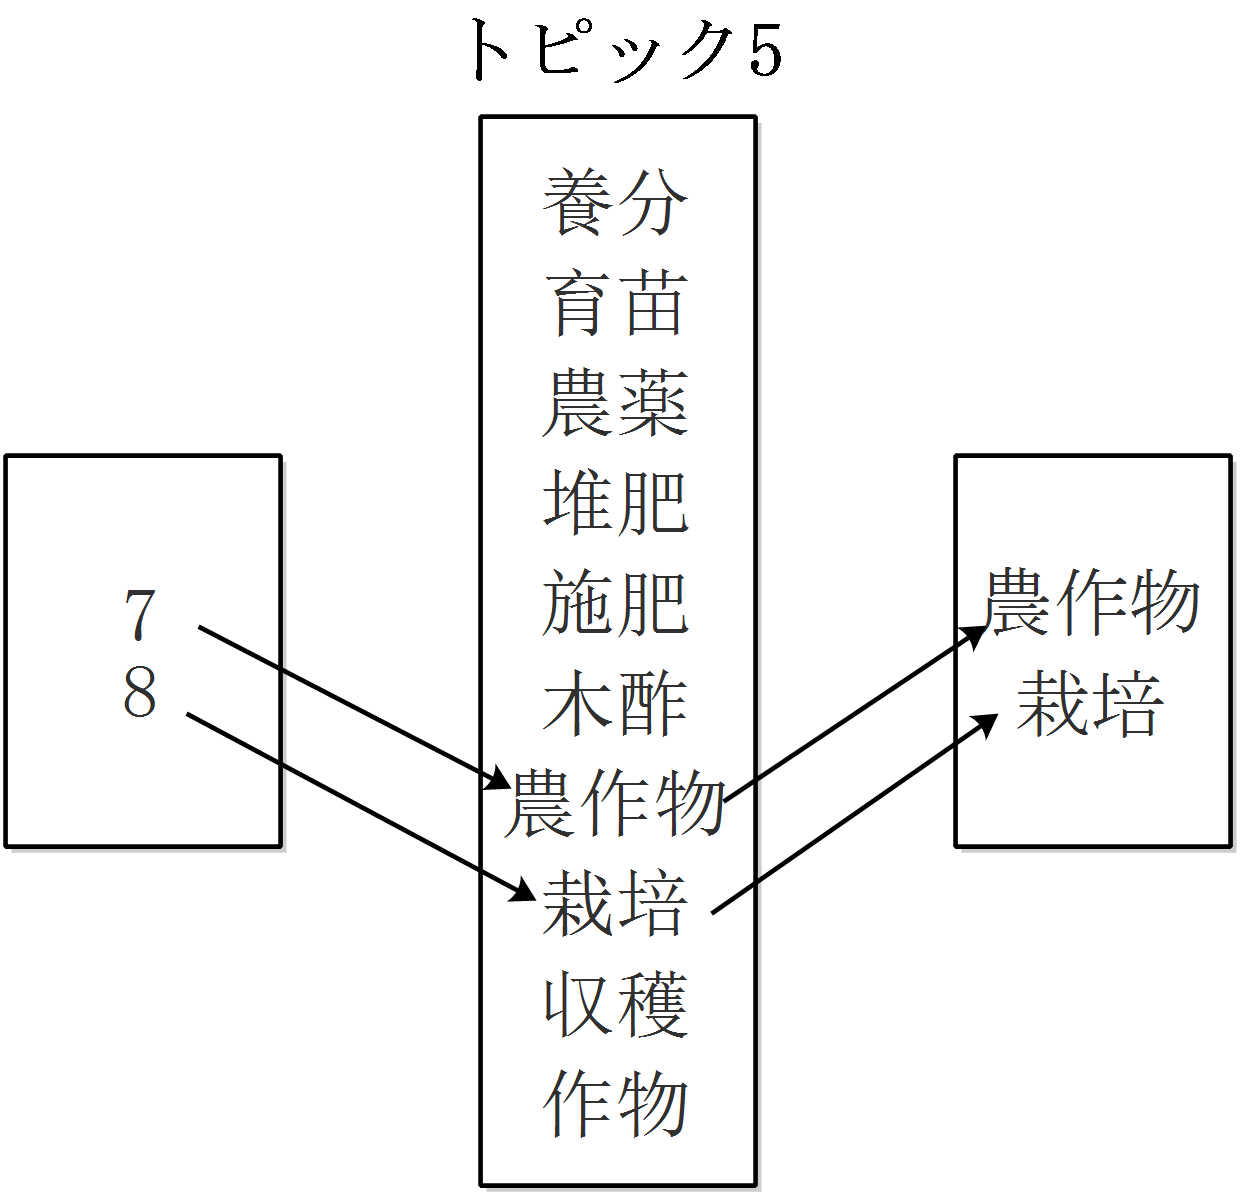
\includegraphics[width=0.9\textwidth,natwidth=310,natheight=299]{tv2.png}
 \caption{数字ベクトル質問化関数$NtW$の例}
 \label{fig:tv2}
 \end{minipage}
 \end{figure}
 \section{質問者が検索したいトピックを曖昧化する質問曖昧化}\label{s:AAAA}
 検索したいトピックを曖昧化する質問曖昧化(QOT)は以下の特徴を持つ.
 まず,トピック出現頻度で質問者が興味あるトピックを特定することを防ぐためにQOTは事前にトピックをグループにし,
 質問者が検索したいトピックが属するトピックグループにある他のトピックをダミートピックとする.
 次に真の質問が同じ単語を含むとき, ダミー質問も同様に同じ単語を含むようにする.

 それを実現するために提案手法では単語ベクトルを用いた.
 単語ベクトルに同じ順番を持つ単語がその単語ベクトルを持つトピックに対して同じ様な関連値を持つと考えられ,
 同じ数字ベクトルで表わせる質問もその質問が属するトピックに対して同じ様な関連値を持つと考えられる.
 したがって,単語ベクトルを通じて違うトピックに属するが似たような特徴を持つ質問を作ることができ,
 メイントピック攻撃に対応できると考えられる.
 
 $TG$をトピックをグループにする関数とし,次のことが成り立つとする.
 \begin{enumerate}
 \renewcommand{\labelenumi}{(\roman{enumi})}
 \item $\forall t \in T,TG(t) \subset T$ 
 \item $\forall t' \in TG(t),TG(t') = TG(t)$
 \end{enumerate}
 
 QOTの質問生成メカニズムが次とおりである:
 \begin{enumerate}
 \renewcommand{\labelenumi}{(\roman{enumi})}
 \item 質問$q$のメイントピック$t_1 = \delta_{SA}(q)$を計算する. 
 \item トピック$t_1$が属するトピックグループ$TG(t_1)$を定める.
 \item 質問$q$を数字ベクトル$v = WtN_{SA}(q,t_1)$にする.
 \item 質問グループを$G = \{NtW(v,t)|t \in TG(t_1)\}$とし,サーバに提出する.
 \end{enumerate}

 質問者がトピック$t_1$に対して一連の質問を提出するを例としてQOTの安全性を分析する.
 トピック$t_1,t_2, \dots ,t_n$が1つトピックグループに属すると仮定する.
 質問者がメイントピックが$t_1$である質問$q^1,q^2, \dots , q^m$をQOTを用いて質問グループ$G_1,G_2, \dots , G_m$に曖昧化する.
 メイントピックが一致する質問ペア間のDice係数がメイントピックが一致ではない質問ペア間のDice係数より大きいと
 SimAtt2で保存した$m$個の質問列が$t_1,t_2, \dots ,t_n$と1対1に対応することが考えられる.
 トピック$t_i$と対応する質問列を$Pu[i]$,
 質問グループ$G_j$の中の$t_i$に属する質問を$q^j_i$とする.
 質問グループ$G_k$に対してSimAtt2攻撃するとき,
 質問ログに存在する任意の質問グループ$G_i$に対して
 $\forall 0 < i < k, coef(q^i,q^k) = coef(q^i_2,q^k_2) = \dots = coef(q^i_n,q^k_n)$
 となりDice係数が同じである質問ペアが存在し,
 $sim_{q^k,Pu[1]} = sim_{q^k_2,Pu[2]} = \dots = sim_{q^k_m,Pu[m]}$
 となるため,質問列との類似度も同じであり,
 SimAtt2での攻撃が無効になる.

 しかし,質問者が1つトピックに対して検索すると限りない.
 特に特許検索の場合はいくつの関係性が強い分野について検索することが多い.
 例えばスマートフォンメーカー企業がスマートフォン通信(Hセクション電気)の特許を検索した後に
 スマートフォン本体の生産装置(Bセクション処理操作)の特許を検索することも考えられる. 
 分野は違うが,同じスマートフォン関する特許であるため,
 2つの質問間の関連値が高いと考えられる.
 HDGAではハッシュ関数でトピックをグループにしているが,各トピック間の関係を配慮していない.
 1つトピックグループ内のトピック間の類似度がQOTのSimAtt2に対する安全性を影響すると考えられる.

 トピックは単語との関連値で表し,一列に並べられないため,
 ETSQが単語をバケットにすると同じようにトピックをグループにするができない.
 本論文では各トピックとの関連値が上位1000個までの単語をそのトピックを代表する単語集合とし,
 トピックを1000個の単語からなる質問とし,
 Dice係数を用いてトピック間の距離を計算し,
 PDSで紹介した凝集型クラスタリングを用いてトピックをグループにする.
 \ref{s:ex}章ではトピックグループ内のトピック間の類似度が安全性への影響を評価する.

 %また,HDGAは各ダミートピックから単語をランダムに選ぶため,
 %真の質問に含まれている単語は違っても属するトピックは同じなら
 %ダミー質問が同じような性質を持つ.
 %一方,同じ真の質問に対して同じダミー質問を生成することができない.
 %真の質問に含まれている単語という情報を用いてないことがHDGAがSimAttに弱い原因だと考えられる.
 
 \section{質問者が検索したいトピックにおける質問曖昧化}\label{s:BBBB}
 攻撃が質問者の質問ログや質問者が興味を持つ分野など事前知識を持つとき,
 いくらダミートピックを増やしても,
 質問ログと類似度が高い質問や質問者が興味を持つ分野に属する質問などの方法で
 真の質問を簡単に見つかれる.

 質問者が検索したいトピックにおける質問曖昧化(QOI)は単語ベクトルを用いて真の質問を数字ベクトルにし,
 数字ベクトルの各要素に対して雑音を加え,
 ダミー質問にする.

 
 \section{データベース分割}
 IPCコードを用いることにより特許データベースを分野ごとに子データベースに分割することができる.
 分割したデータベース各々に対して同じような信憑性を持つ質問を提出すると真に検索したいデータベースを隠すことができると考えられる.
 しかし,LSAやLDAなど意味分析手法を用いて得たトピックは人の手によって分類された子データベースと1対1に対応できない.
 本論文では検索サーバが第\ref{s:sm}章で紹介した$tfidf$を用いて単語と各子データベースの関連値を計算し,子データベースごとに単語ベクトルを作り,
 質問者に公開する.

 質問者が検索するときは,
 真の質問を検索したい子データベースの単語ベクトルを用いて数字ベクトルにし,サーバに提出する.
 そして,サーバは質問者からもらった数字ベクトルを各子データベースに送り,
 各子データベースの単語ベクトルを用いて質問にし,各子データベースを検索する.
 図\ref{fig:dbb}はこの流れを表している.
 質問者は自ら意味分析を用いてダミー質問を作る必要がない.
 また,検索サーバでは各子データベースを並列で検索することができるため,
 ダミー質問による応答時間の増加を削減する. 
 最後,質問者はサーバからもらった各子データベースの検索結果から真の子データベースの検索結果を利用する.
 
 \begin{figure}
 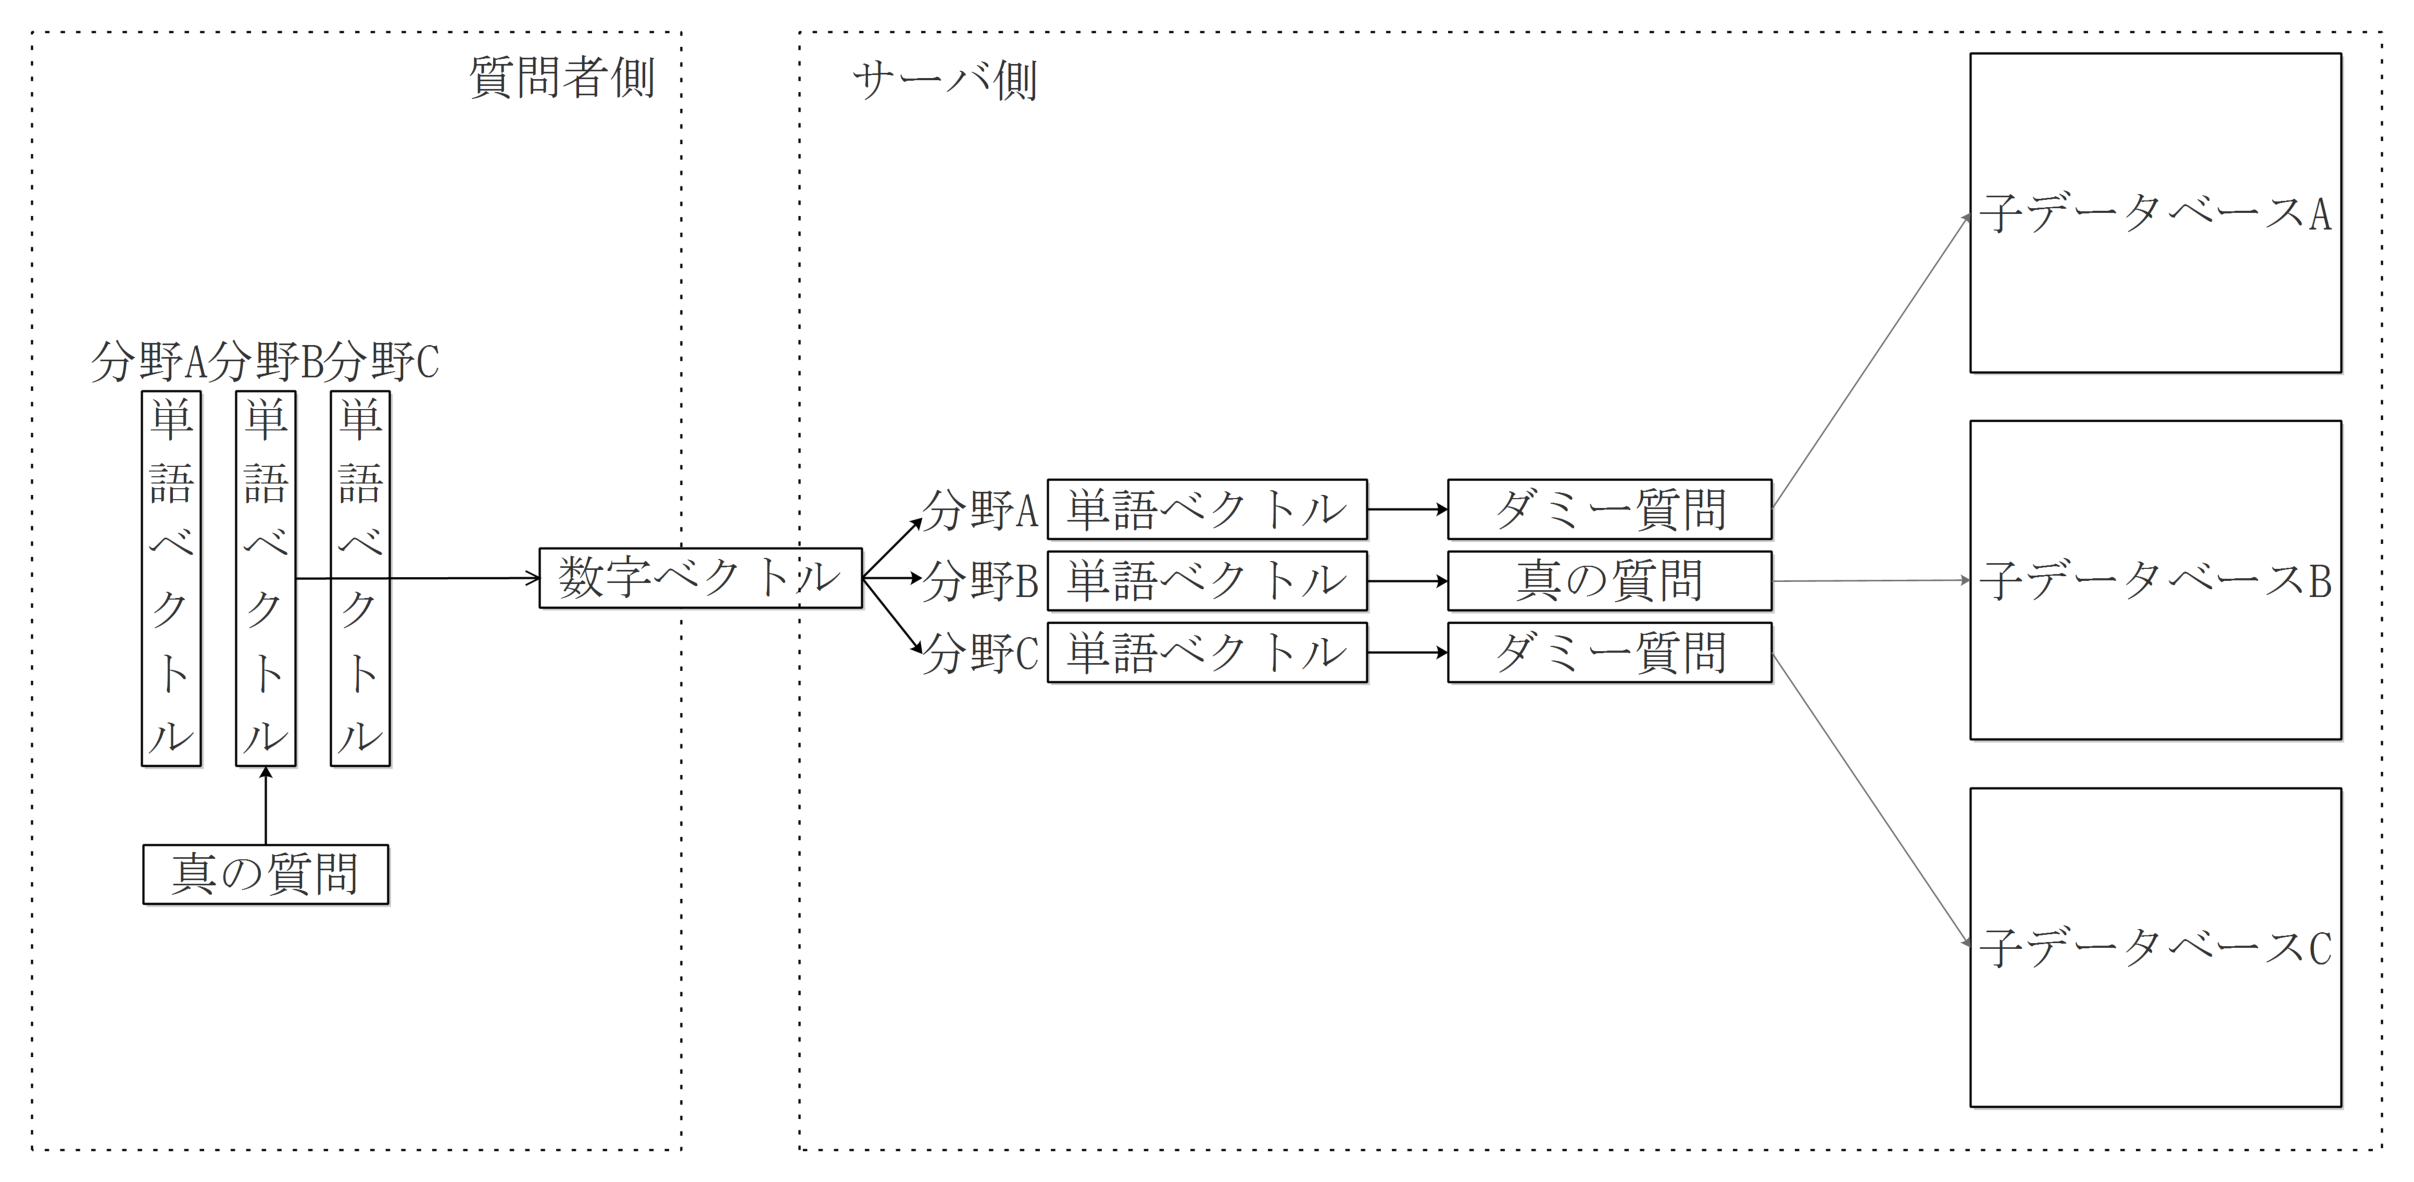
\includegraphics[width=0.9\textwidth,natwidth=997,natheight=476]{dbb.pdf}
 \caption{データベース分割の流れ}
 \label{fig:dbb}
 \end{figure}
 
 データベース分割では他の曖昧化と違って全ての子データベース,
 あるいはトピックについて質問を提出する.
 そのため,質問者がHセクションの特許について質問$q_1$を検索した後に
 Bセクション特許について質問$q_2$を検索するとき,
 Hセクションに属するダミー質問$q'_2$が必ず同じ質問グループに存在し,
 Bセクションに属する真の質問$q_2$より前に提出したHセクションに属する質問$q_1$との類似度が高いと考えられる.
 SimAtt2では意味的に近い一連の質問を真の質問とするため,
 真の質問$q_1$と$q_2$ではなく
 より意味的近い質問ペア$q_1$と$q'_2$を1つの質問列にする.
 そのため,データベース分割手法は
 SimAtt2に対してよりいい防御ができると考えられる.

 \chapter{評価実験} \label{s:ex}
 本章ではNTCIR-6\cite{NTCIR6}の無効資料調査タスクのデータセットを用いて特許検索における既存手法ETSQ,HDGAと提案手法を安全性を評価する.
 評価実験は全て8個の2.5GHz CPUと61GBメモリをもつAWS Linuxインスタンスで実行する.

 \section{文書集合と質問集合}
 NTCIR-6は国立情報学研究所(NII)から配布されている
 1993年から2002年まで発行分の約350万文書がある日本公開公報を検索対象である文書集合とする.
 無効資料調査タスクの質問は特許庁の審査感が拒絶した特許文書の一般的に最も重要な第一請求項を用いる.
 無効資料調査タスクの参加者は請求項を解析し単語を重要度を計算する手法や検索された文書の一部を用いて検索質問拡張を行う手法など
 を用いて検索精度を上げる.
 しかし,本論文は検索結果の精度ついて評価していないため,単純に請求項から名詞を抽出し検索質問をする.
 また第\ref{s:sm}章で説明したように本論文はIPCコードを用いて特許文書を623個のIPCサブクラスに分類する.
 文書集合と質問集合の詳細は表\ref{tab:data}に示す. 

 \begin{table}[!hbp]
 \center
 \begin{tabular}{|c|c|}
 \hline
 重複を除いた単語数 & $2,973,096$  \\
 文書数 & $3,496,253$ \\
 質問数 & $2,908$ \\
 質問平均単語数 & $21.0$ \\
 国際特許分類数 & 623 \\
 \hline
 \end{tabular}
 \caption{データセット}
 \label{tab:data}
 \end{table}

 意味分析手法について,
 LSAとLDAは共に64トピックに設定する.
 特許文集集合の単語数が多く,全ての単語に対してLDAを行うことは困難であるため,
 本論文では各IPCサブクラスとの$tf\text{-}idf$値が上位1000個にある単語32524個に対してLDAを行う.
 評価実験で用いる質問の単語の$99.0\%$が上記32524個単語の中である.
 
 本章で用いる略称は表\ref{tab:abbr}

 \begin{table}[!hbp]
 \center
 \begin{tabular}{|c|c|c|}
 \hline
 手法 & 略称  & 節\\
 \hline
 潜在意味分析 & LSA & \ref{s:LSA}節 \\
 潜在ディリクレ配置法 & LDA & \ref{s:LDA}節 \\
 質問者のプライバシーを保護する質問加工法 & ETSQ & \ref{s:ETSQ}節 \\
 質問意図を曖昧化するキーワード検索 & HDGA & \ref{s:HDGA}節 \\
 質問者が検索したいトピックを曖昧化する質問曖昧化 & QOT & \ref{s:AAAA}節 \\
 質問者が検索したいトピックにおける質問曖昧化 & QOI & \ref{s:BBBB}節 \\
 メイントピック攻撃 & MTA & \ref{s:MTA}節 \\
 事前情報がある場合の類似度攻撃 & SimAtt & \ref{s:SimAtt}節 \\
 事前情報がない場合の類似度攻撃 & SimAtt2 & \ref{s:SimAtt2}節 \\
 \hline
 \end{tabular}
 \caption{略称}
 \label{tab:abbr}
 \end{table}

 \section{メイントピック攻撃}
 \subsection{質問者のプライバシーを保護する質問加工法}
 ETQSでは任意2つの単語バケットで全ての同じ位置の単語ペア間の意味的距離の差が小さいなら,
 真の質問の単語が意味的に近いときあるいは一つのトピックに集中したとき,
 バケットの中のダミー単語も同じように一つのトピックに集中すると考えるため,
 本論文はSegSzを一番単語ペア間の意味的距離の差を小さくでき,攻撃しづらいと考えた1に設定する.
 またWordnetは人の手によって作成されたため,$27\%$の質問単語がWordnetに存在しない,
 評価実験ではWordnetに存在しない単語を抜いて攻撃する.
 LSAとLDAを用いてメイントピック攻撃した結果が図\ref{fig:mt1}で表している.
  
 \begin{figure}
 \begin{minipage}[t]{0.5\linewidth}
 \centering
 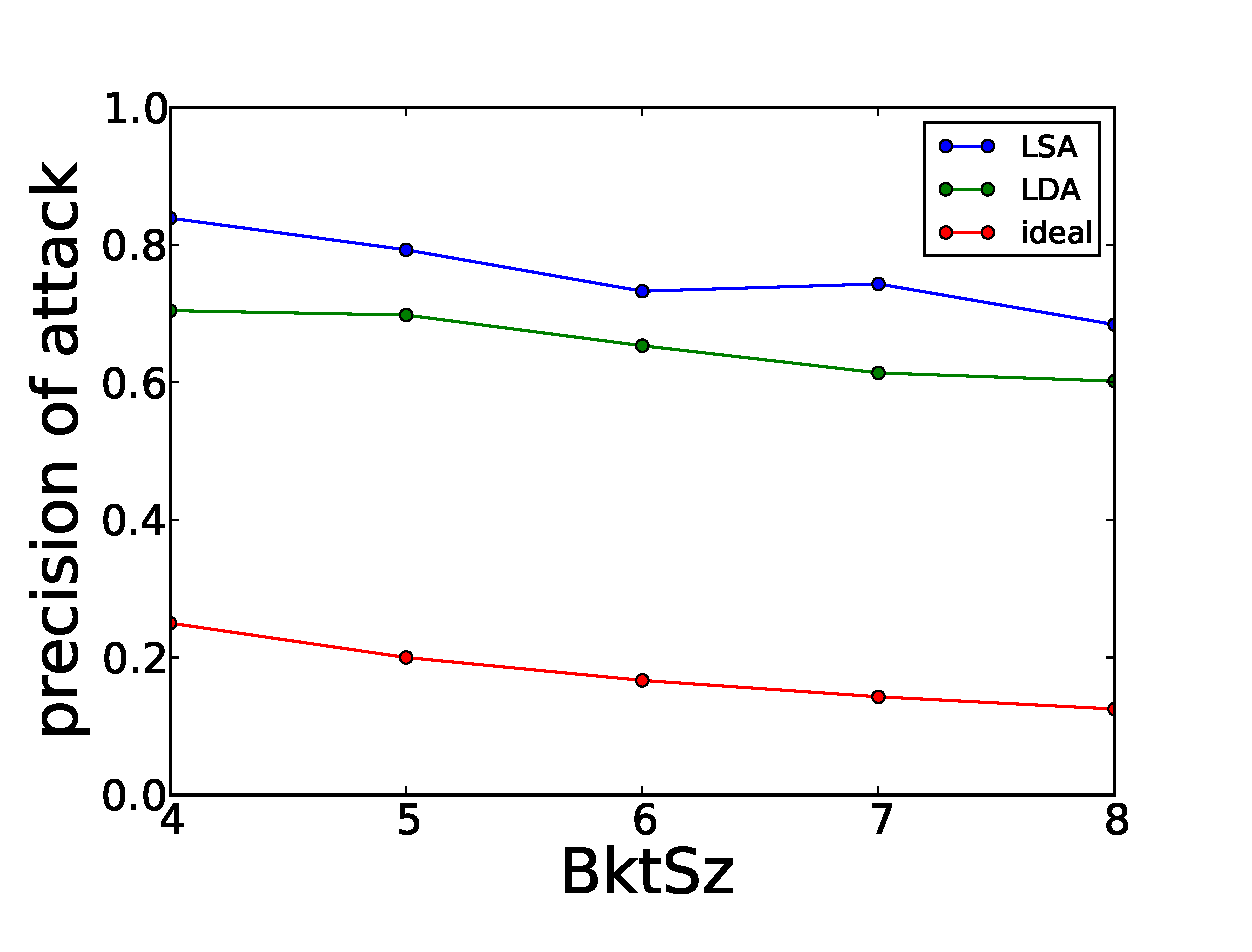
\includegraphics[width=0.9\textwidth]{ETSQ1.eps}
 \vspace{5em}
 \caption{単語バケットに対してメイントピック攻撃の成功率}
 \label{fig:mt1}
 \end{minipage}%
 \begin{minipage}[t]{0.5\linewidth}
 \centering
 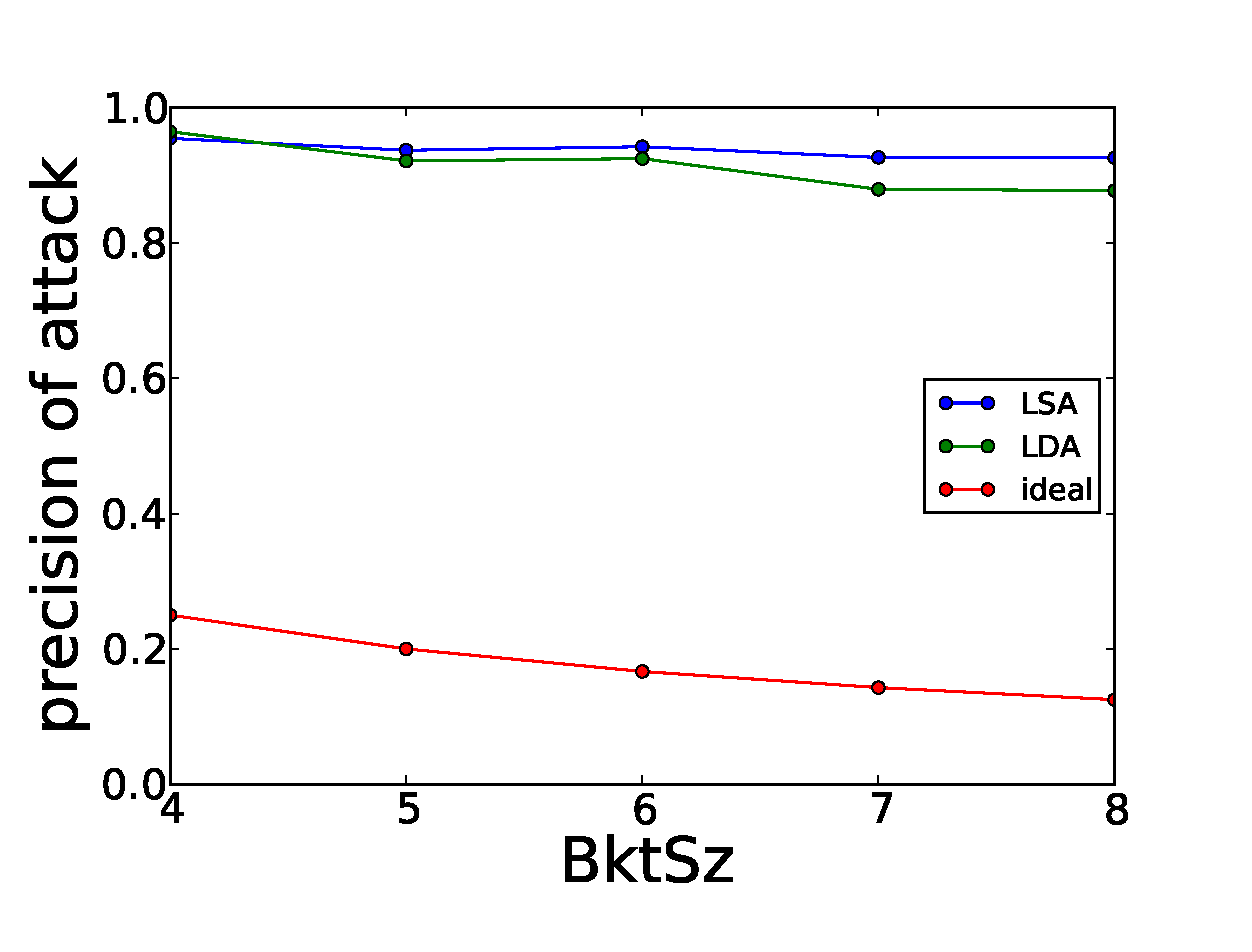
\includegraphics[width=0.9\textwidth]{ETSQ2.eps}
 \vspace{5em}
 \caption{加工した質問のメイントピックと真の質問のメイントピックが一致する確率}
 \label{fig:mt2}
 \end{minipage}
 \end{figure}
 
 単語ごとに$7$個のダミー単語を加えても$60\%$以上の確率で真の質問の単語を見破られる.
 図\ref{fig:mt2}が加工した質問のメイントピックと真の質問のメイントピックが一致する確率を表している.
 ダミー質問の単語を1つトピックに集中しないと真の質問のメイントピックを隠すことが困難であると考えられる.
 
 \subsection{質問意図を曖昧化するキーワード検索}
 HDGAはダミートピックの決定し,ダミートピックにおける単語の出現率でランダムに単語を選び真の質問と同じ長さのダミー質問を作る.
 攻撃者が質問者と同様にLDAを用いてメイントピック攻撃する結果が図\ref{fig:mt:HDGA}に示す.
 ここでmaxは質問グループの中で自分のメイントピックの関連値$Pr[\delta_{LDA}(q)|q]$が一番高い質問$q$が真の質問である確率で
 minは質問グループの中で自分のメイントピックの関連値$Pr[\delta_{LDA}(q)|q]$が一番低い質問$q$が真の質問である確率である.
 
 \begin{figure}
 \begin{minipage}[t]{0.5\linewidth}
 \centering
 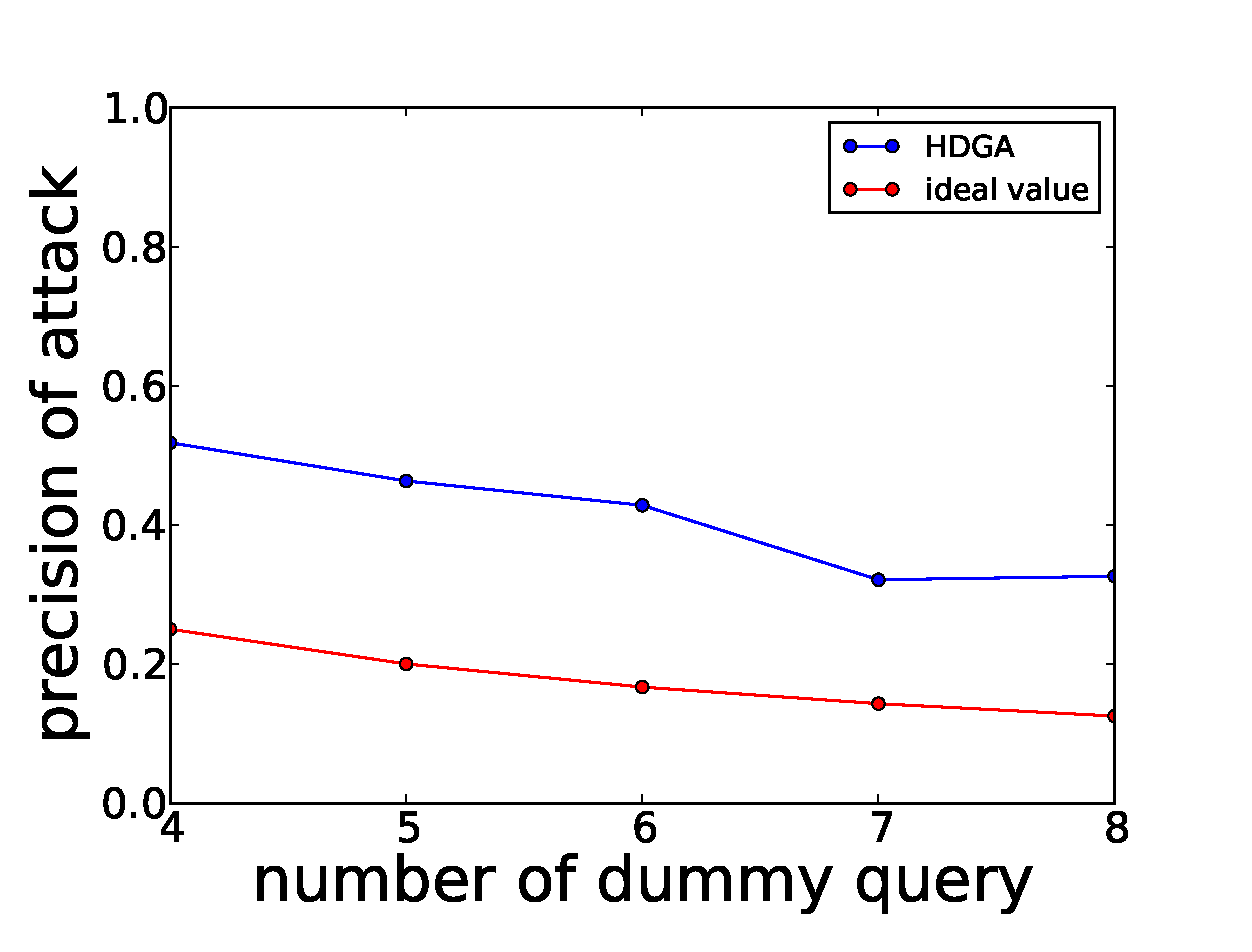
\includegraphics[width=0.9\textwidth]{HMD.eps}
 \vspace{5em}
 \caption{HDGA vs. MTA}
 \label{fig:mt:HDGA}
 \end{minipage}%
 \begin{minipage}[t]{0.5\linewidth}
 \centering
 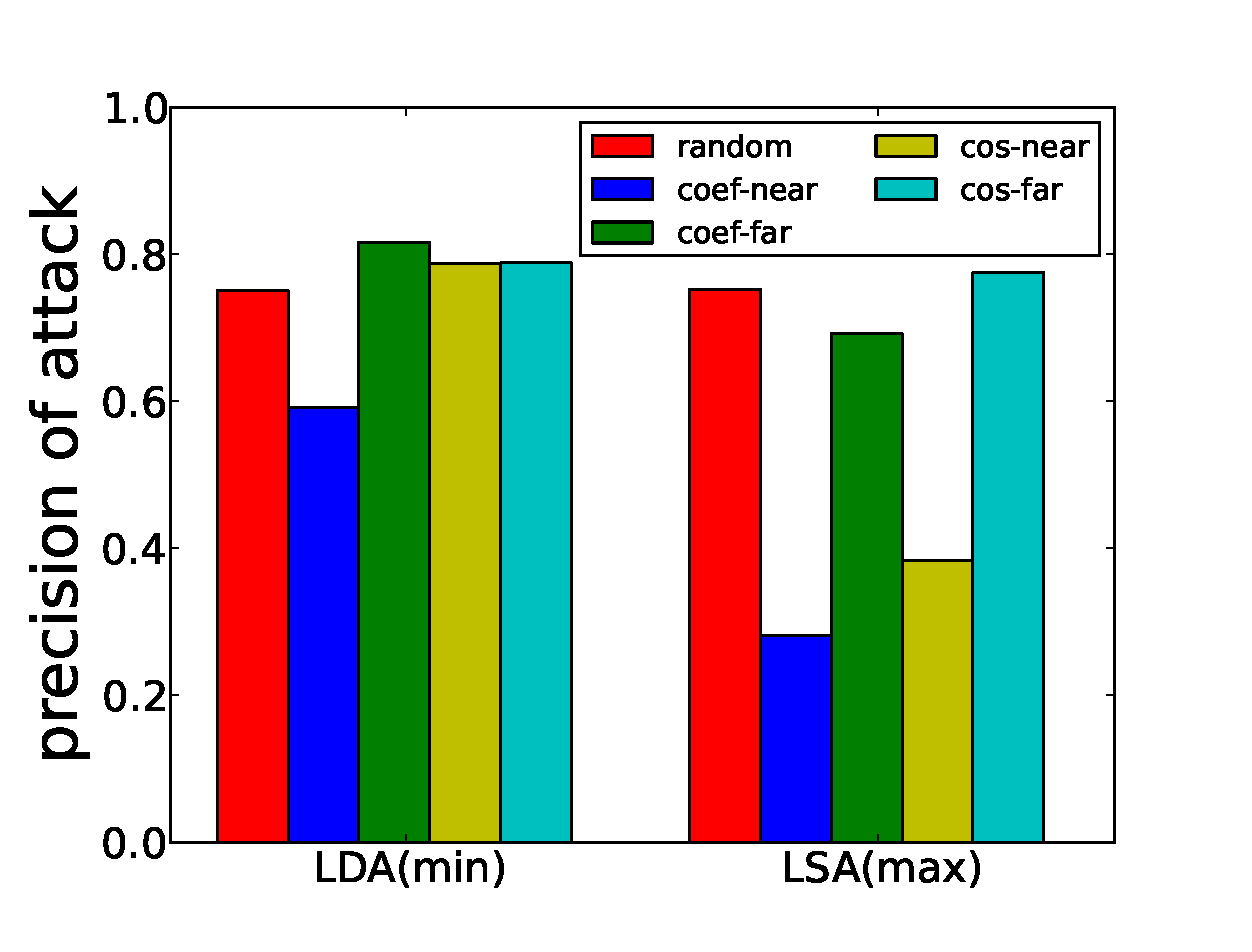
\includegraphics[width=0.9\textwidth]{AAAA1.eps}
 \vspace{5em}
 \caption{QOT vs. MTA}
 \label{fig:mt:AAAA}
 \end{minipage}
 \end{figure}

 HDGAではダミートピック$t$を決定し,ダミートピックから$Pr[w|t]$に基づいてランダムに単語を選択するため,
 各質問$q$に対してトピック$\delta_{LDA}(q)$における確率$Pr[q|\delta_{LDA}(q)] = \prod_{w \in q}Pr[w|\delta_{LDA}(q)]$の差が少ない.
 しかし,同じ文書に出現する確率が高い単語を用いた真の質問$q$が出現する確率$Pr[q]$がダミー質問が出現する確率より大きくなるため,
 真の質問とその質問のメイントピックの関連値$Pr[\delta_{LDA}(q)|q]=\frac{Pr[q|\delta_{LDA}(q)]Pr[\delta_{LDA}(q)]}{Pr[q]}$が一番低くなると考えられる.
 本節ではLDAを用いてメイントピック攻撃するときは関連値$Pr[\delta_{LDA}(q)|q]$が一番低い質問を真の質問とする.

 %また,今までの既存研究では攻撃者が質問者と同じの意味分析手法を用いると仮定するが,

 \subsection{質問者が検索したいトピックを曖昧化する質問曖昧化}
 攻撃者が質問者と同じ意味分析手法を用いてQOTに対してメイントピック攻撃を行うとき,
 1つトピックグループ中のトピック間の距離の影響は図\ref{fig:mt:AAAA}に示す.
 ここで1つの真の質問に対して3つのダミー質問を加えるとする.
 第\ref{s:sm}章で説明したように,coef距離はトピックの代表単語集合間のDice係数で,
 cos距離はトピックの代表単語集合を意味分析手法を用いて得たトピックベクトル間のcos距離である.

 LDAを用いるときはHDGAと同じように真の質問とその質問のメイントピックの関連値が一番低くなる確率が高い.
 意味的に近いトピックをダミートピックとにすることにより,
 トピックの出現率$Pr[t]$間の差と単語ベクトルで同じ順番の単語$|w|$がそのトピックにおける出現率$Pr[w|t]$間の差を小さくなり,
 HDGAによりいい結果を得ることができたと考えられるものの,
 真の質問が出現する確率とダミー質問が出現する確率間の差を無くすことができないため,
 理想値でメイントピック攻撃を防ぐことができないと考えられる.
 
 LSAを用いて意味的に近いトピックと1つトピックグループにする場合は最も良い結果となった.
 意味的に近いトピックをダミートピックとすることにより,
 真の質問が属するトピック$t$とダミー質問が属するトピック$t'$の単語ベクトルに同じ順番$i$を持つ単語$w_i = wvec_{SA}(t)[i]$と$w'_i = wvec_{SA}(t')[i]$
 がそのトピックとの関連値$rscore_{SA}(w_i,t)$と$rscore_{SA}(w'_i,t')$間の差を無くすことが考えられ,
 LSAでは質問が出現する確率を分析できないため,
 質問の出現率の差で真の質問を見つけることができないことが考えられる. 

 また,直接に単語を用いて距離を計算する場合が単語の曖昧性をなくす意味分析手法を用いる場合よりいい結果を得たのは
 特許文書は曖昧性を生じないように単語を選んだためと考えられる.

% 1つトピックグループ中のトピック間の距離
% が
% 真の質問とダミー質問の検索結果の一致する割合
% に対する影響は\ref{}に表している.
% 真のトピックと意味的に近いトピックをダミートピックにしても質問意図の安全性に影響しないと考えられる.

 \subsection{質問者が検索したいトピックにおける質問曖昧化} 
 QOIに対してはQOTを攻撃するときと同じように
 攻撃者が質問者と同じ意味分析手法を用いて評価実験した結果は図\ref{fig:mt:BBBB}に示す.
 QOIは真の質問と同じトピックに属する似たような関連値を持つダミー質問を生成するが,
 LDAを用いるQOIはQOTで意味的に近いトピックを1つのトピックグループにするときと同じような安全性を得る.
 同じトピックに属する質問をダミー質問にしても,
 真の質問の出現確率とダミー質問の出現確率間の差を無くすことができないと考えられる.

 \begin{figure}
 \begin{minipage}[t]{0.5\linewidth}
 \centering
 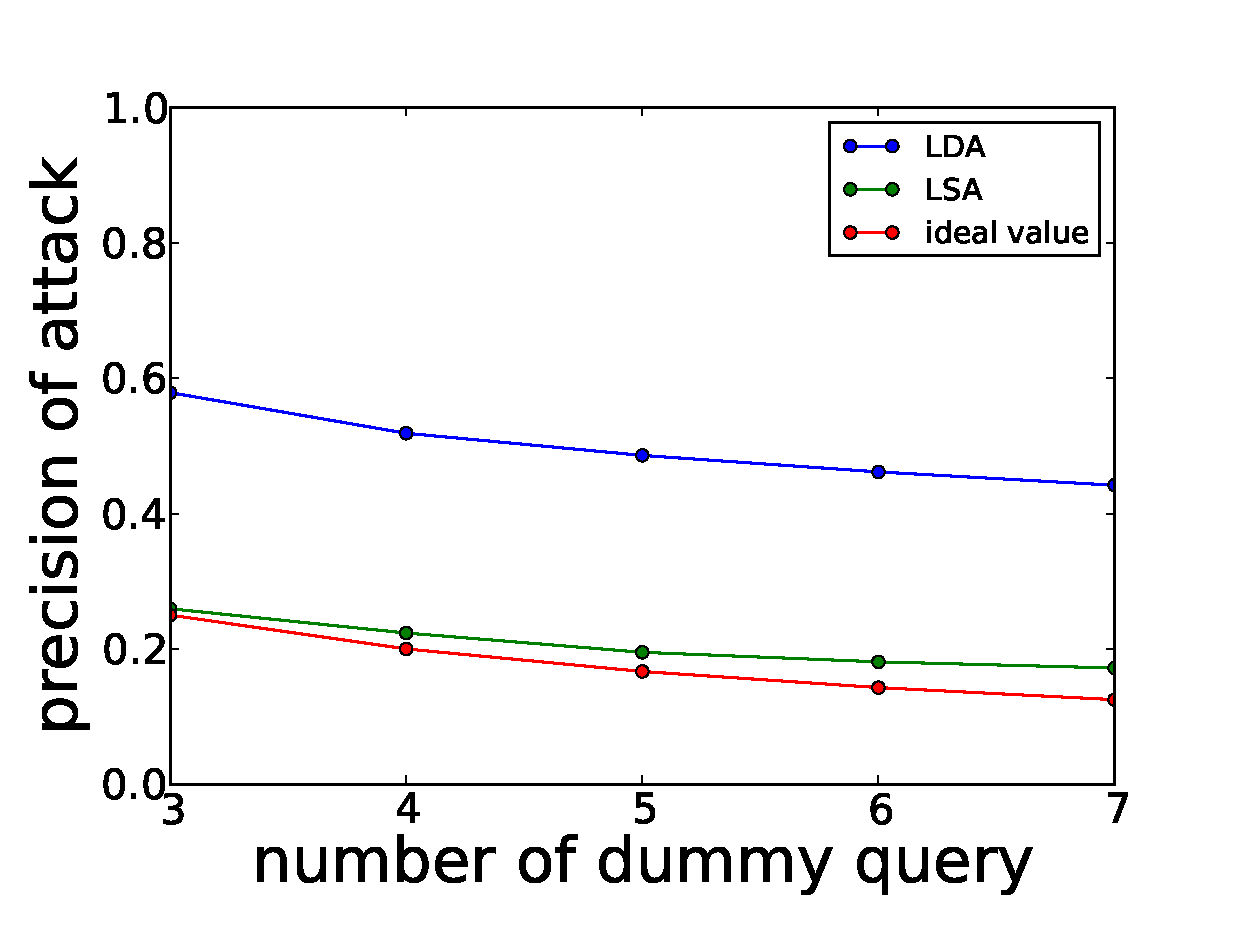
\includegraphics[width=0.9\textwidth]{BBBB1.eps}
 \vspace{5em}
 \caption{QOI vs. MTA}
 \label{fig:mt:BBBB}
 \end{minipage}%
 \begin{minipage}[t]{0.5\linewidth}
 \centering
 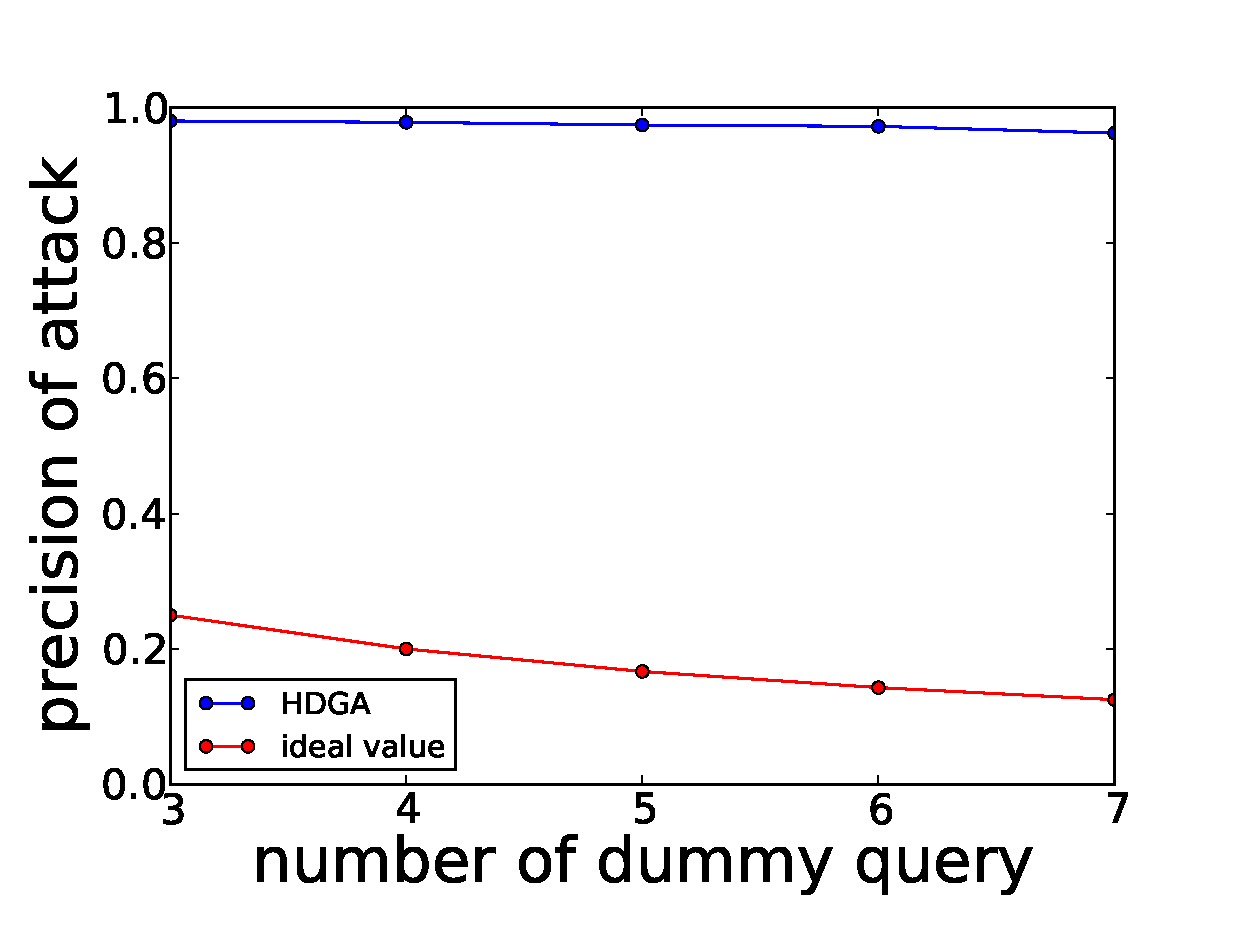
\includegraphics[width=0.9\textwidth]{HDGA1.eps}
 \vspace{5em}
 \caption{HDGA vs. SimAtt2}
 \label{fig:s2:HDGA}
 \end{minipage}
 \end{figure}

 QOTの場合と同様にLSAを用いるQOIに対してメイントピック攻撃する場合は真の質問を見破られない.
 
 \section{事前情報がない場合の類似攻撃}

 無効資料タスクで用いた質問は審査感が拒絶した特許文書から抽出されたものであるため,
 特許文書にあるほかの情報も利用できる.
 本論文では1つ企業が出願した特許文書から抽出された質問を
 1人の質問者が提出した質問にする.
 SimAtt2の評価実験では5個以上の質問を提出した質問者72人が提出した1562個質問について攻撃する.

 ETQSでは1回の検索に対して1つ加工した質問しか提出しないため,
 類似攻撃は対応できない.

 \subsection{質問意図を曖昧化するキーワード検索}
 図\ref{fig:s2:HDGA}に示すようにHDGAではダミー質問の個数を7個まで増やしても$96.2\%$で真の質問を見つける.
 \ref{s:SimAtt2}節で説明したようにHDGAは質問が提出した一連の質問グループの質問間の関連値を配慮していないためと考えられる.

 \subsection{質問者が検索したいトピックを曖昧化する質問曖昧化}
 QOTに対してSimAtt2を行うとき1つトピックグループ中のトピック間の距離の影響は図\ref{fig:s2:AAAA}に示す.
 LSAを用いて意味的に近いトピックをダミートピックとすることにより,
 第\ref{s:AAAA}節で議論したように質問者が意味的に近いが同じトピックに属しない質問を連続提出した影響を減らし,
 HDGAに比べてよりいい結果を得ることができたが,
 3つのダミー質問に対して$66.8\%$で真の質問を見つけることは安全であると言えない.


 \begin{figure}
 \begin{minipage}[t]{0.5\linewidth}
 \centering
 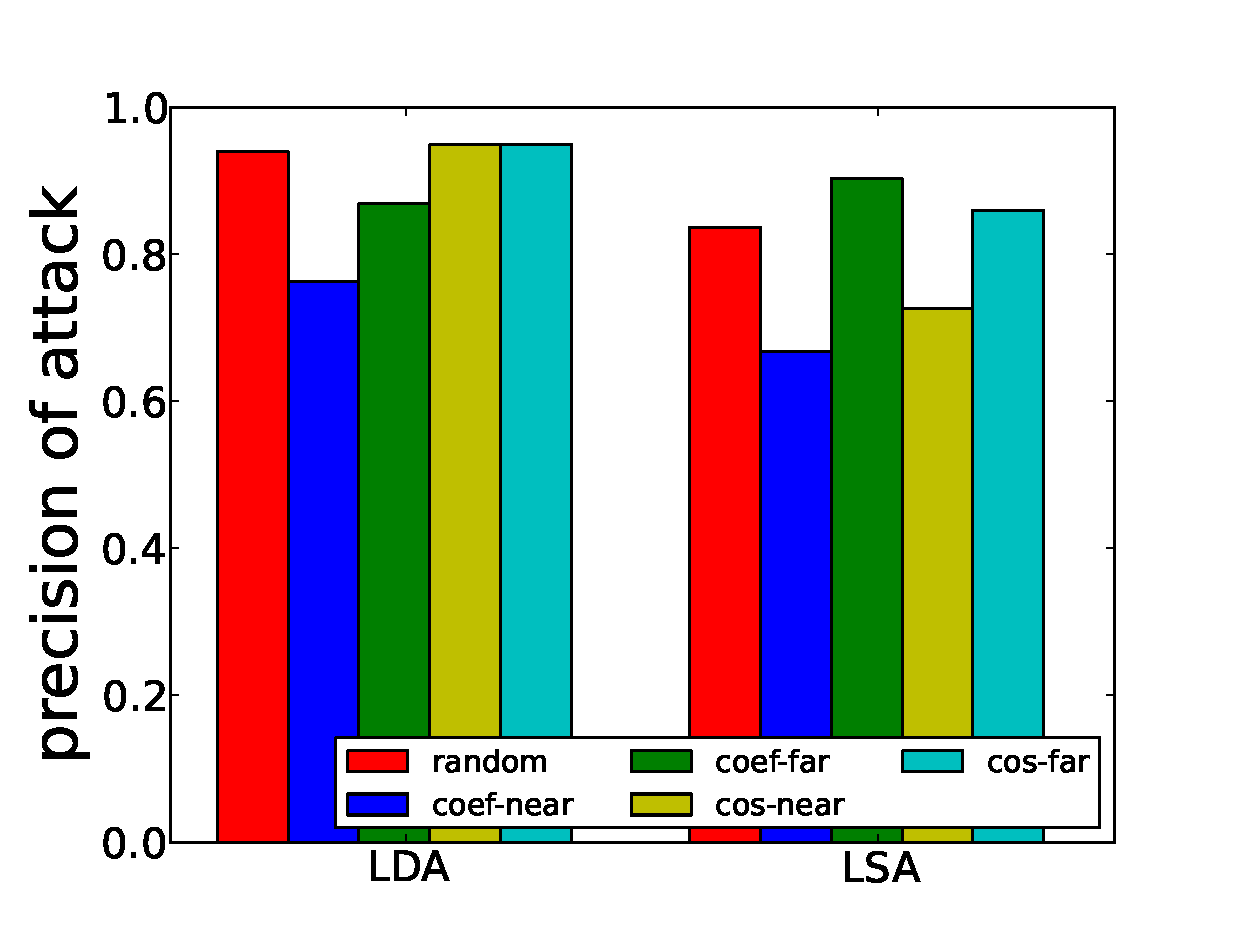
\includegraphics[width=0.9\textwidth]{AAAA2-2.eps}
 \vspace{5em}
 \caption{QOT vs. SimAtt2}
 \label{fig:s2:AAAA}
 \end{minipage}%
 \begin{minipage}[t]{0.5\linewidth}
 \centering
 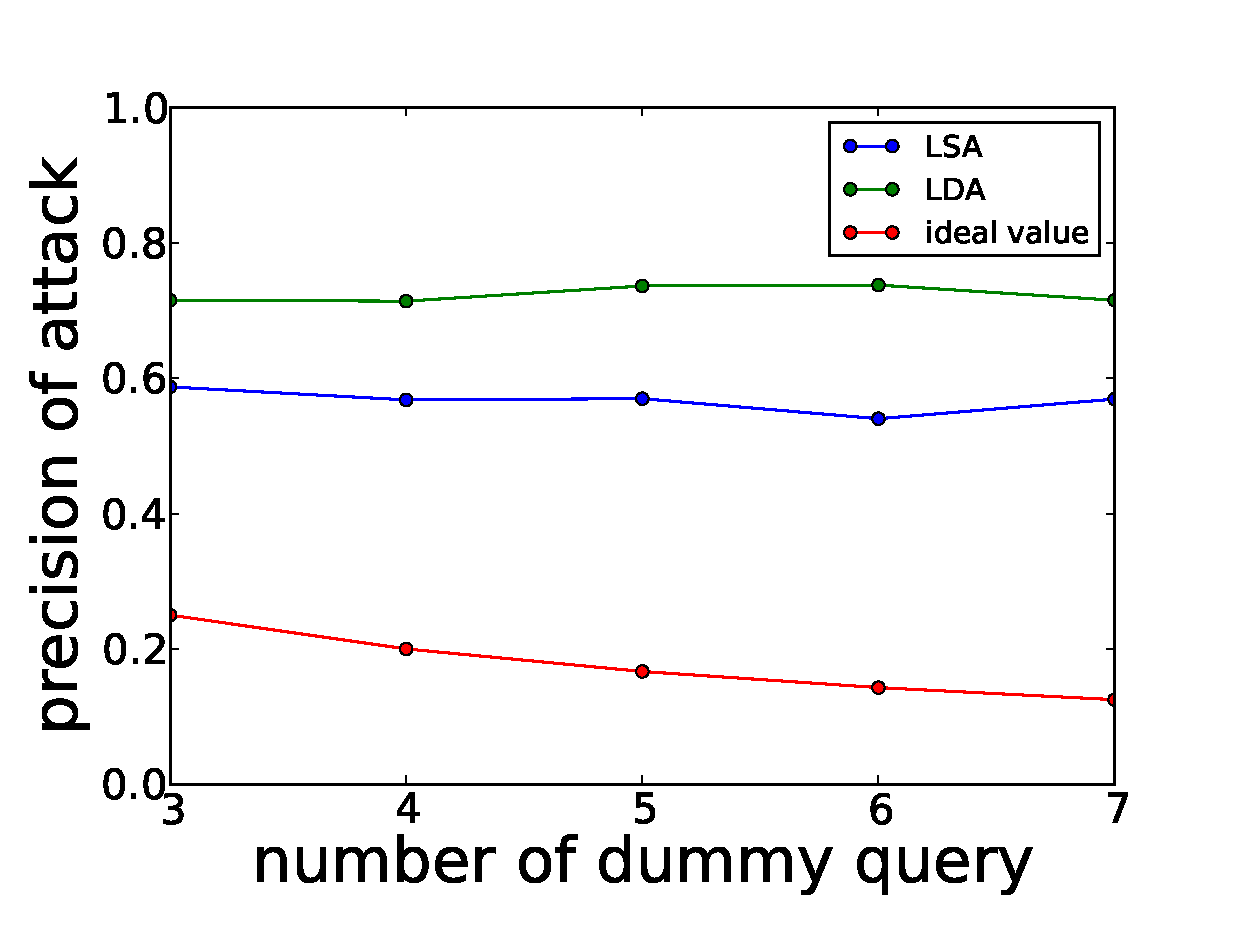
\includegraphics[width=0.9\textwidth]{BBBB2.eps}
 \vspace{5em}
 \caption{QOI vs. SimAtt2}
 \label{fig:s2:BBBB}
 \end{minipage}
 \end{figure}

 \subsection{質問者が検索したいトピックにおける質問曖昧化} 
 QOIでは1つ質問グループの中の質問全部1つのトピックに属し,
 真の質問が意味的に近いときダミー質問も意味的に近いと考えられる.
 しかし,特許文書では曖昧性を生じないように同じものを指すときは同じ単語を用いるため,
 同じ質問が提出した質問が意味的に近いだけではなく
 同じ単語を用いる確率も高い.
 そのため,
 単語の重複率で質問間の類似度を計算する類似度攻撃は
 一般なウェブ検索に攻撃するときよりいい効果を得たと考えられる.
 その結果を図\ref{fig:s2:BBBB}に示す.
 
 \section{事前情報がある場合の類似攻撃}
 類似攻撃の評価実験ではSimAtt2で用いた各質問者の質問からランダムに3つを選び,
 その質問者が攻撃者に知られている質問ログとし,
 その質問ログを用いて類似攻撃する.
 
 実験結果は図\ref{fig:s1}に表している.
 QOTとQOIではSimAtt2に対して一番いい結果を得た意味分析手法LSAとcoef距離が近いトピックグループを用いた.

 評価実験で用いた質問では質問の$22\%$の単語が攻撃者に知られている質問ログに存在するため,
 単純な質問曖昧化手法で類似攻撃から質問意図を守ることができないと考えられる.

 \begin{figure}
 \begin{minipage}[t]{0.5\linewidth}
 \centering
 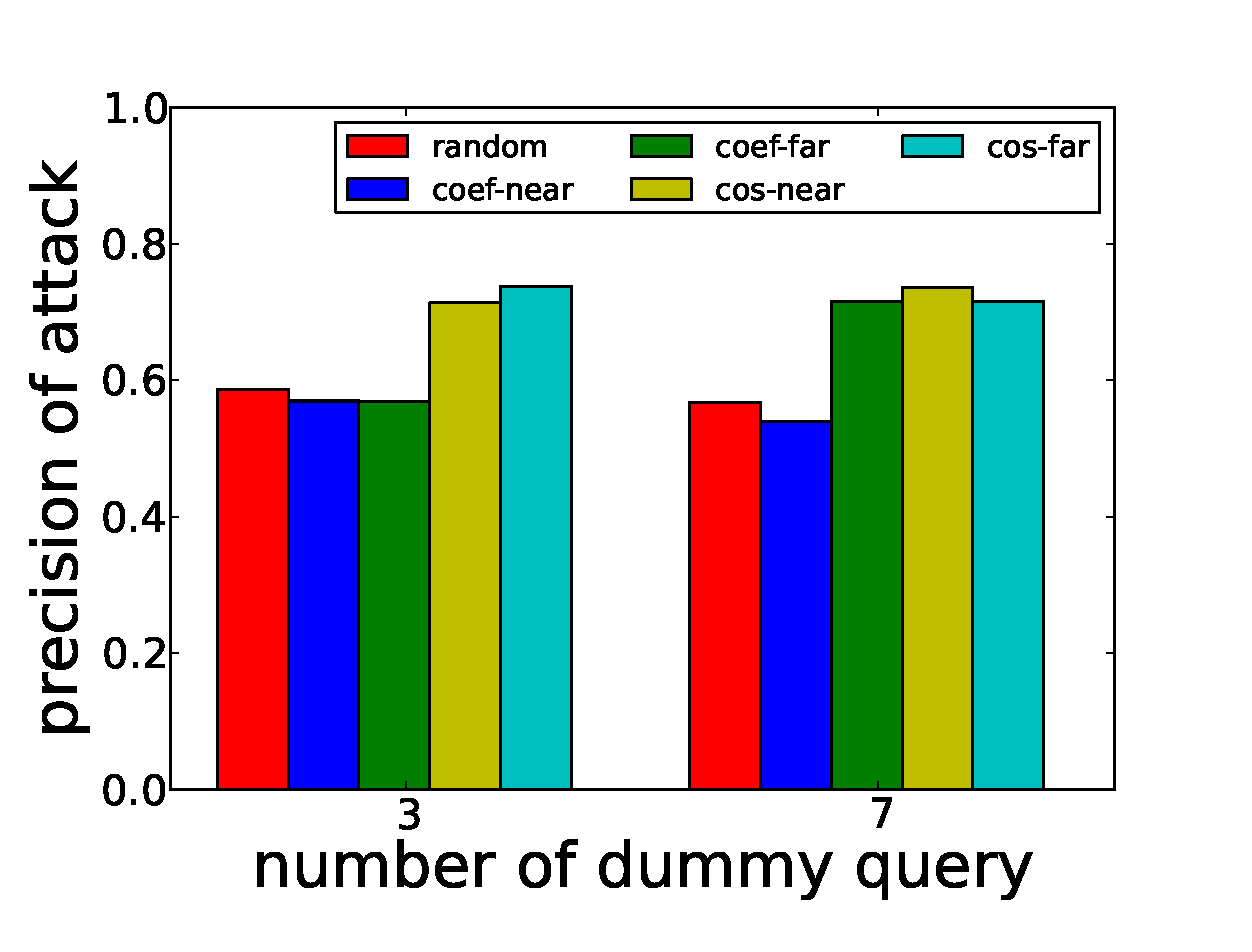
\includegraphics[width=0.9\textwidth]{SA2.eps}
 \vspace{5em}
 \caption{SimAtt}
 \label{fig:s1}
 \end{minipage}%
 \begin{minipage}[t]{0.5\linewidth}
 \centering
 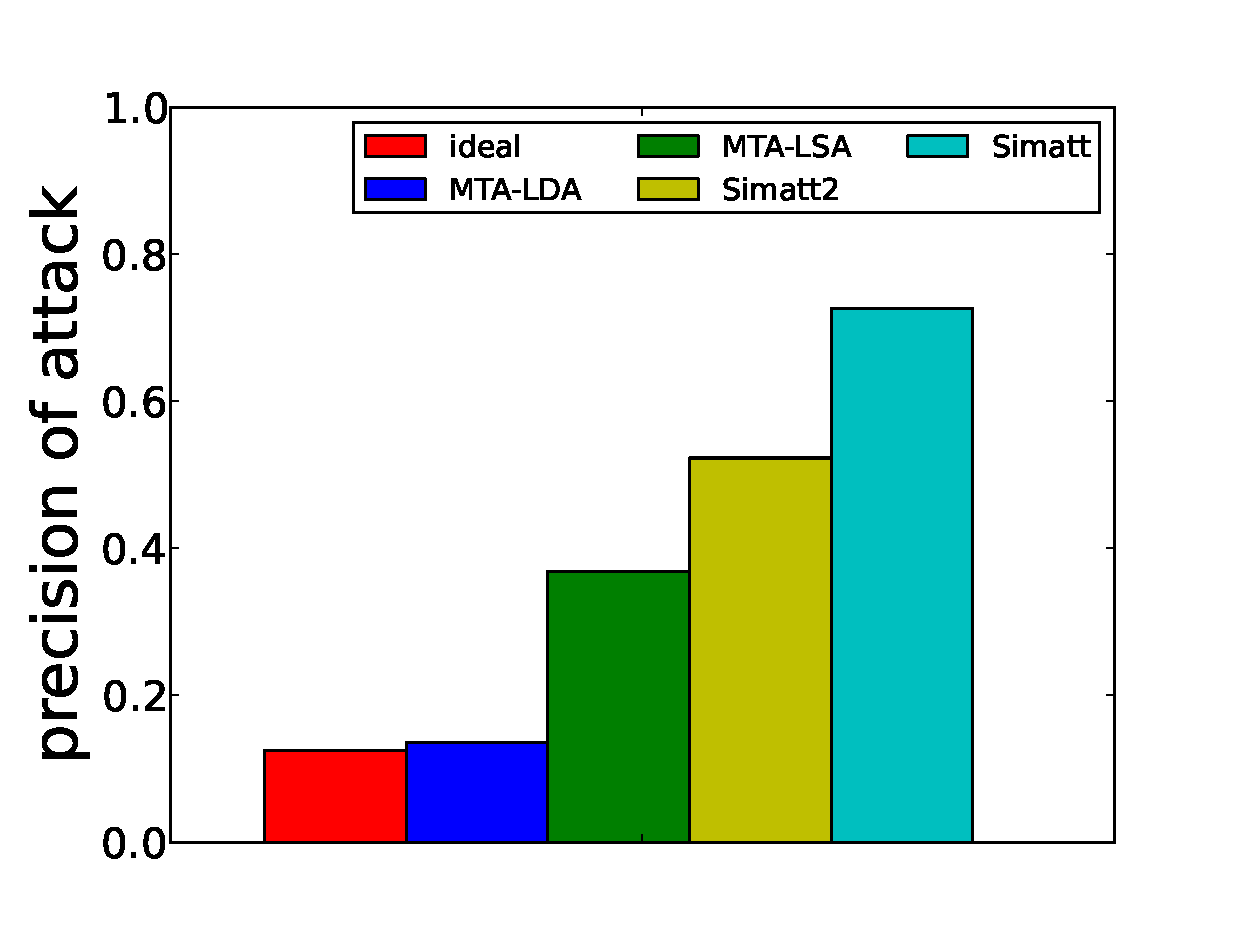
\includegraphics[width=0.9\textwidth]{DS.eps}
 \vspace{5em}
 \caption{データベース分割}
 \label{fig:ds}
 \end{minipage}
 \end{figure}

  
 \section{データベース分割}
 本論文では国際特許分類の一番上の階層の8個のセクションを用いて
 特許文書を8個の子データベースに分割し,評価する.
 評価実験結果は図\ref{fig:ds}に表している.
 
 データベース分割はLDAを用いたメイントピック攻撃MTA-LDAに対しては理想値に近い高い性能を出している.
 このことから,
 子データベースにおけるtf-idf値に基づいて作られたダミー質問$q'$がその質問のLDAにおけるメイントピック$\delta_{LDA}(q')$における出現率$Pr[q'|\delta_{LDA}(q')]$
 が真の質問$q$出現率$Pr[q|\delta_{LDA}(q)]$より低いと考えられるものの,
 ダミー質問$q'$の出現率$Pr[q']$も真の質問より低いため
 メイントピックとの関連値$Pr[\delta_{LDA}(q)|q]$と$Pr[\delta_{LDA}(q')|q']$が近くなったと考えられる.
 このことを確かめるため真の質問とダミー質問の出現率を調べた.
 $36.49\%$の真の質問の出現率がダミー質問の出現率より高い結果となった.
 また,LSAを用いたメイントピック攻撃MTA-LSAは$36.90\%$で真の質問を見つける.
 このことから,単語と子データベース間のtfidf値が単語とトピックの関連値を表せると考えられものの,
 子データベースの数が少ない,
 LDAとLSAを用いて得たトピックと対応できないため,
 LDAとLSAにおける多次元なトピック空間を完璧に記述することができないと考えられる.
  
 類似攻撃に対しては全てのトピックに対して質問を提出することよりトピック間の差よる
 質問間の類似度の差と質問と質問が属するトピックの関連値の差が小さくなるが,
 トピック数が減らしたため,
 同じトピックに属するダミー質問が意味的に遠くなり,
 攻撃されやすくなると考えられる.  

 \section{交差攻撃}

 今までの評価実験では既存研究と同様に
 攻撃者と質問者が同じ意味分析手法を用いた.
 しかし,LDAでは1つのトピック集中している単語はLSAを用いても
 同じく1つのトピック集中すると限らない.
 本節では攻撃者が質問者と違う意味分析手法を用いてメイントピック攻撃を行った.

 \begin{figure}
 \begin{minipage}[t]{0.5\linewidth}
 \centering
 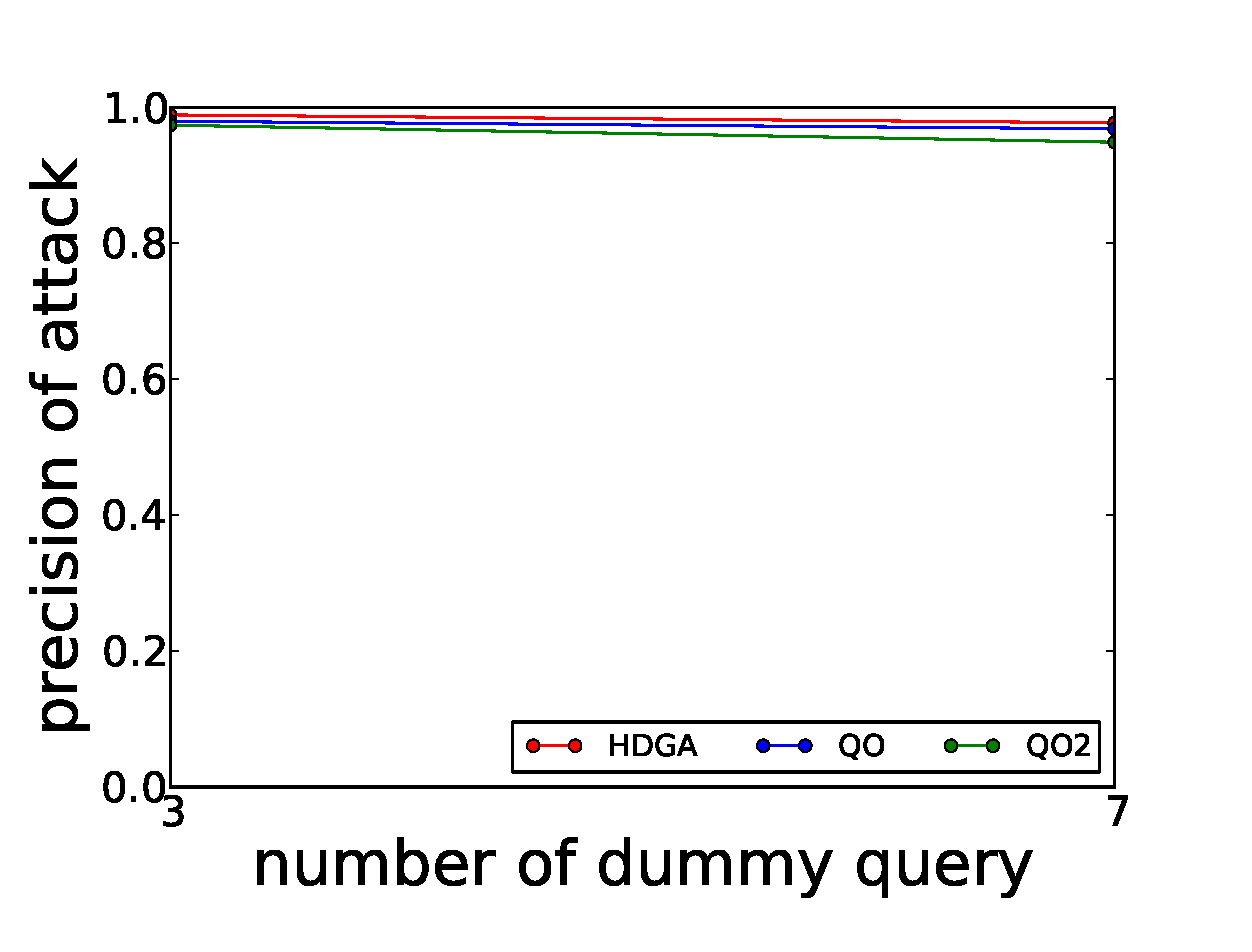
\includegraphics[width=0.9\textwidth]{CROSS1.eps}
 \vspace{5em}
 \caption{質問者:LDA vs. 攻撃者:LSA}
 \label{fig:cr1}
 \end{minipage}%
 \begin{minipage}[t]{0.5\linewidth}
 \centering
 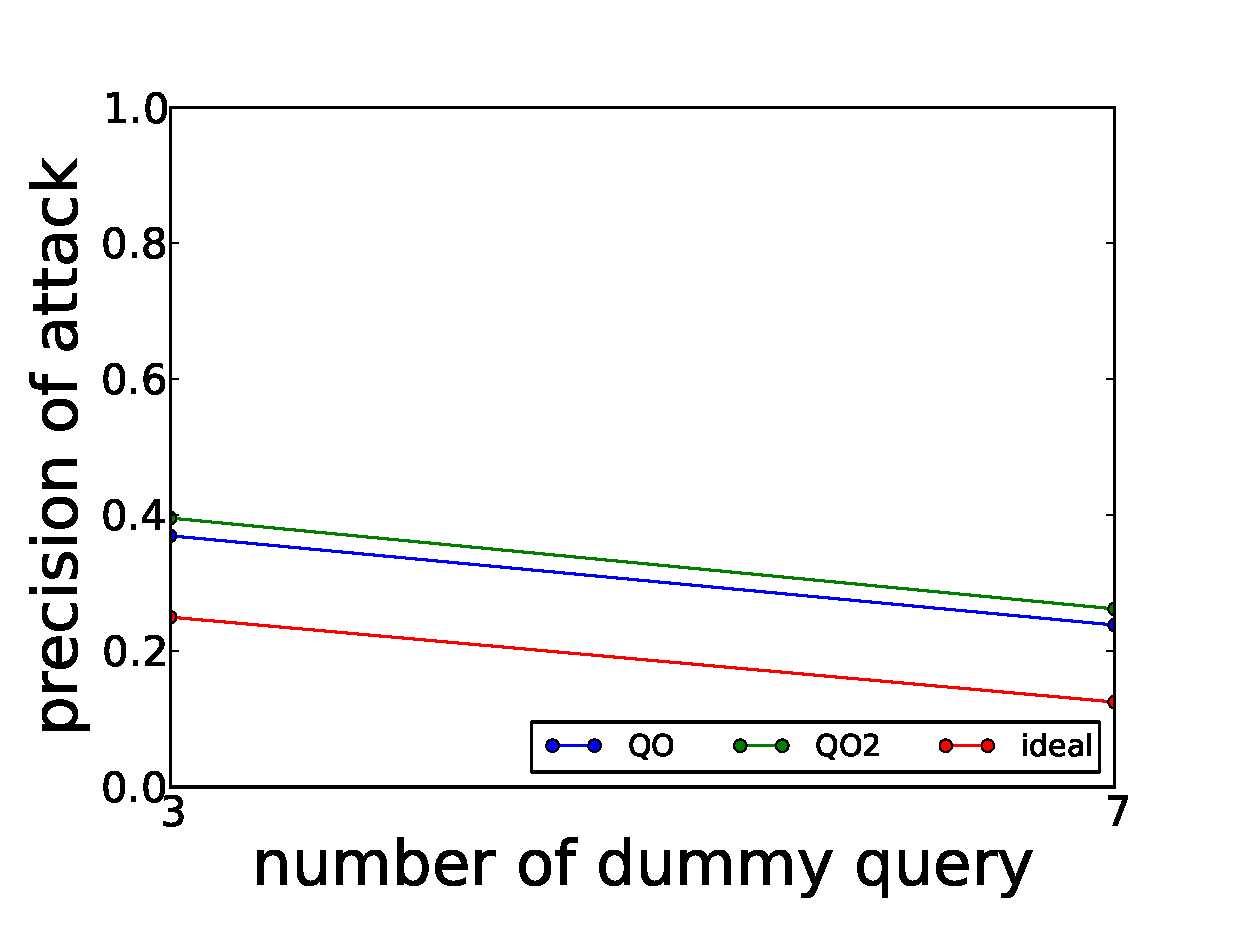
\includegraphics[width=0.9\textwidth]{CROSS2.eps}
 \vspace{5em}
 \caption{質問者:LSA vs. 攻撃者:LDA}
 \label{fig:cr2}
 \end{minipage}
 \end{figure}

 図\ref{fig:cr1},\ref{fig:cr2}は交差攻撃の結果を表している.
 LDAモデルのトピックとLSAモデルのトピックは一対一に対応できないため,
 両方とも攻撃者が質問者と同じ意味分析手法を用いた場合より良い攻撃結果となった.
 ダミートピックからランダムに生成したダミー質問は真の質問のように複数の意味分析に対応できる強さを持たないと考えられる.
 また,LSAを用いた場合,LDAを用いた結果を大きく上回っている.
 このことから,単語数が多いが文章数が少ないコーパスに対して意味分析する場合は
 LSAがLDAより良い効果を出すと考えられる.
 
 \begin{table}[!hbp]
 \center
 \begin{tabular}{|c|c|c|c|c|c|}
 \hline
   & \multicolumn{5}{|c|}{攻撃者} \\
 \hline
 \multirow{7}*{質問者} & & MTA-LSA & MTA-LDA & SimAtt2 & SimAtt \\
 & ETSQ & 83.9 & 68.4 & x & x \\
 & HDGA & 98.9 & 83.1 & 98.0 & \\ 
 & QOT-LSA &  & 39.6 & 66.8 &\\
 & QOT-LDA & 98.0 & & 76.3 &\\
 & QOI-LSA & 25.9 & 37.0 & \\
 & QOI-LDA & 97.4 & 57.9 &\\
 & データベース分割 & 36.9 & 13.6 & 52.3 & 72.7 \\
 \hline
 \end{tabular}
 \caption{表記法}
 \end{table}
 
 
 \chapter{おわりに}
 本論文では特許検索における曖昧化検索手法と攻撃手法を提案し,既存の曖昧化検索手法対してに実データを用いて手法の安全性を評価した.
 評価実験結果により,提出しようとしている質問のみからダミー質問を生成する手法は
 質問ログを持つ攻撃者から質問意図を保護することが困難であると考えられる.
 また,どのような意味分析手法においても同じような強さを持つダミー質問を生成することが今後の課題として挙げられる.

 \backmatter% ここから後付
 \chapter{謝辞}%%%%%%%%%%%%%%% 謝辞 %%%%%%%
 本論文は多くの方々のご指導ご支援の下,書き上げることができました.
 指導教員の中川先生には,多くのとこをご教授してくださりました.
 テーマの設定のしかたや関連研究の調べ方,論文の書き方など研究活動に必要な多くのことを学びました.
 荒井助教授には研究テーマの選別,実験データの作成などで大変お世話になりました.
 
 また,同研究室の後輩,同期,先輩方一同にも,発表等において毎回数多くのご指摘を頂きました.
 特に博士の小宮山さんは研究だけではなく,その他生活全般についてお世話になっていたものと思っています.
 
 以上簡単ではありますか,まとめて感謝の意を記させていただきたいと思います.
  %\begin{thebibliography}{}%%%% 参考文献 %%%
  % \bibitem{}
  %\end{thebibliography}
  %\bibliographystyle{ieicetr}%           BibTeX を使う場合

  \bibliography{thesis}% BibTeX を使う場合

  \appendix% ここから付録 %%%%% 付録 %%%%%%%

  %\chapter{}
  \end{document}

 \subsection{プライバシー分析}
 PDSでは真の質問$q_u$の代わりに真の質問と一番類似した質問$q_c$を含んでいる質問セットをサーバに送る.
 $q_c$が真の質問の大半な結果を検索できると考えられ,質問セット中の他の質問をダミー質問に見なす.
 そのため,このメカニズムは検索の精度と再現率に影響を大きく与える.
 また,質問の長さの増加と伴って質問の可能な組み合わせが指数的に増加するため,実際には特許検索など長い質問が多いテキスト検索と質問拡張に対応できない.


 

 
 
 攻撃者が質問者と違う意味分析手法を用いて攻撃する結果はは\ref{}に表している.
 HDGAに対する評価実験と同じように違う意味分析手法を用い,
 トピックの計算方法を変えることより,
 真の質問がの確率で見破られる.
 
  \begin{table}[!hbp]
 \center
 \begin{tabular}{|c|c|}
 \hline
 符号 & 意味 \\
 \hline
 $W = \{1,2,3, \dots ,N\} $ & 単語集合 \\
 $D = \{1,2,3, \dots ,M\}$ & 文書集合 \\
 $K$ & トピック数 \\
 $T = \{1,2,3, \dots ,K\}$ & トピック集合 \\
 $\ell_i = \{t_1,t_2,\dots,K\} $ & 単語$i$のトピックベクトル \\
 $\ell$ & 質問のトピックベクトル \\
 \hline
 \end{tabular}
 \caption{表記法}
 \end{table}
